\chapter{Main Body}
\label{cha:Main Body}


\section{''Pflichtenheft''}
\label{sec:Pflichtenheft}

\subsubsection{Cost}
I've already bought two \acs{devboard}s one of them stays at \acs{tbz} and the other is at home. One of these boards was paid by Mr. Malacarne. Further expenses e.g. the PCB will be paid by me and shouldn't exceed about 50 CHF, as the \acs{hw} isn't that complicated.

\subsubsection{Time}
The majority of the time in the project, I will work at home because it's a rather big project to execute in one semester. I will also have much time in the fall holidays to work on it. The project will approximately take 100h to complete. Also, the more detailed time plan is in chapter [\ref{sec:GANTT Chart}] and sequential 2-week plans in chapter [\ref{sec:Journal}].

\subsubsection{Tools}
To realize this project I will mainly use, the \acs{sw} STM32CubeIDE with \acs{hal}, STM32 CubeProgrammer and Altium Designer. The documentation is written in LaTeX in VSCode. And I'm planning to order the PCB on JLCPCB and will populate and reflow the PCB at ETHZ, where I'm also allowed to use the measurement equipment for the commissioning and miscellaneous measurements.

\subsubsection{Technical Details}
\begin{table}[H]
    \centering
    \label{tab:Technical Details}
\begin{tabular}{||c || c | c | c | c  || c ||} 
 \hline
 value &  min. & typ. & max. & unit & description \\ [0.5ex] 
 \hline\hline
  supply voltage & & 5 & & V & over USB \\ 
 \hline
 curent to measure & 0 & & 1 & A & 2 ranges \\ 
 \hline
 voltage to measure & 0 & & 10 & V & 2 ranges \\ 
 \hline
 com. baud rate & & 115200 & & s\textsuperscript{-1} & UART \\
 \hline
\end{tabular}
    \caption{Technical Details}
\end{table}

\newpage


\section{Extension PCB}
\label{sec:Extension PCB}



\subsection{STMod+}
Interface from DevBoard to Extension PCB. 

\begin{itemize}
    \item 5V Supply
    \item SPI 
    \item I\textsuperscript{2}C
    \item ADC
    \item Interrupt
    \item PWM
    \item GPIOs
\end{itemize}

I will use the STMOD\#14 connection that was intended to use as PWM, as a second ADC input. To measure current and voltage at the same time to later show the power cosumption of the DUT.

\begin{figure}[H]
	\centering
	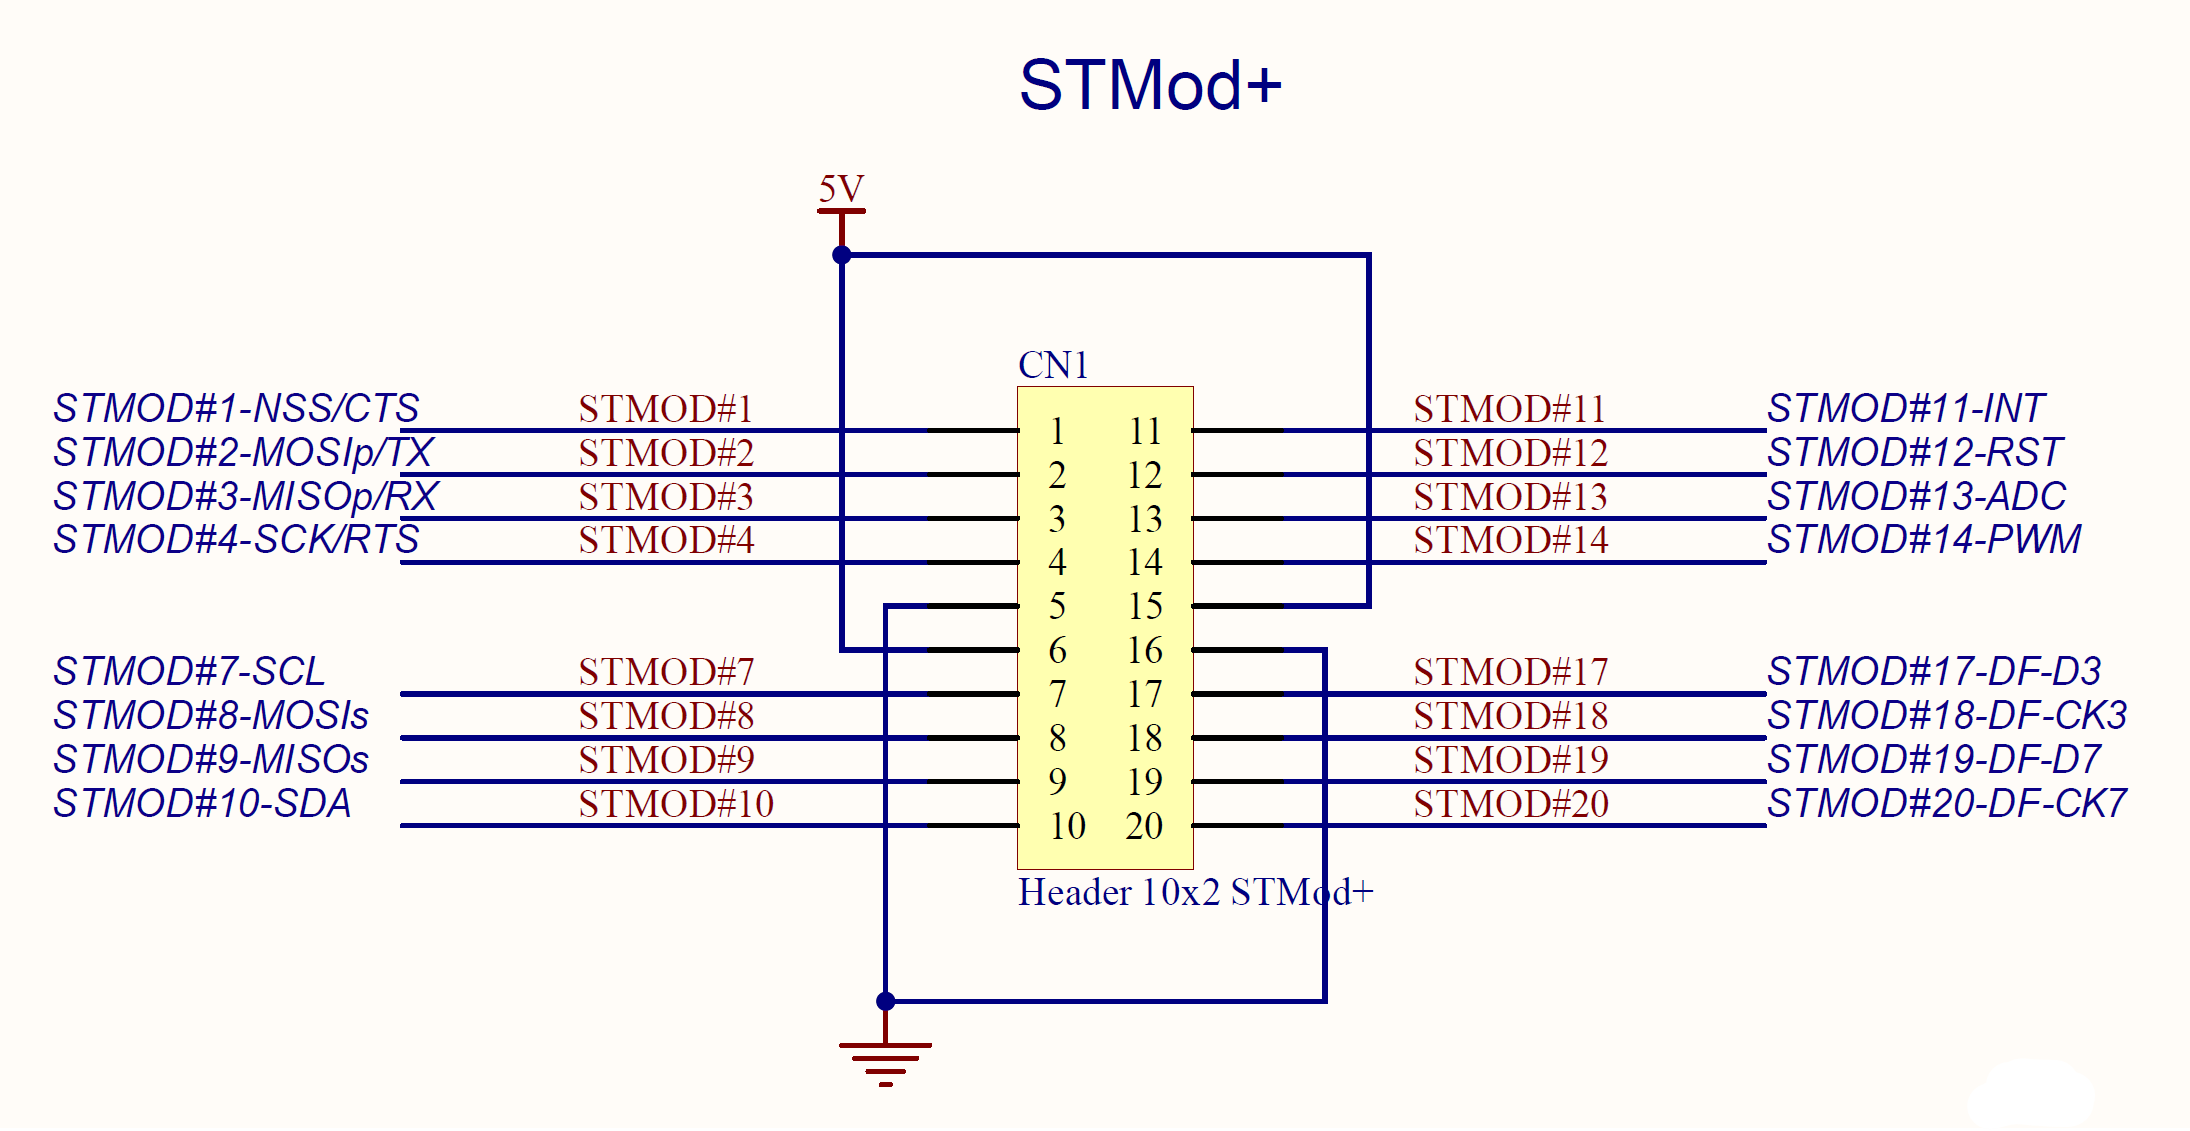
\includegraphics[width=13cm]{Resources/STMOD_Interface.png}
	\caption{STMod+ Interface}
	\label{fig:STMod+ Interface}
\end{figure}




\newpage

\subsection{Hardware concept}

After some thoughts I came up with the following HW concept.


\begin{figure}[H]
	\centering


    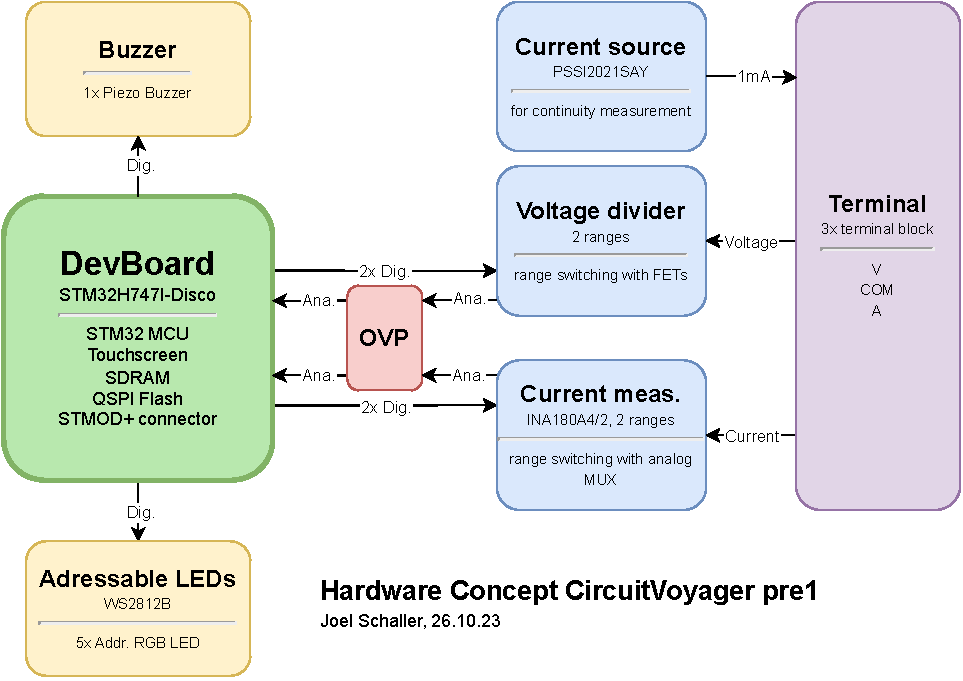
\includegraphics[width=15cm]{../../2_Project_Planning/HW_Concept/Hardware_Concept_CircuitVoyager_pre1.pdf}

    \vspace{0.2cm}

	\caption{Extension PCB HW concept}
	\label{fig:Extension PCB HW concept}
\end{figure}

\subsubsection{Voltage measurement}
To measure voltage, the DUT should be connected to the terminals V and COM. COM is connected internally to device GND. The V terminal is connected to the Voltage divider block. This block divides the input voltage down, so the ADC in the MCU doesn't overshoot. There are 2 ranges to measure voltage, which can be chosen by setting 2 digital outputs, that go from the MCU to the voltage divider. There's also an OVP, to protect the MCU from voltages higher than 3.3V. \cite{DMM_Video_ElectroNoobs}

\subsubsection{Current measurement}
To measure current, the DUT should be connected to the terminals A and COM. COM is connected internally to device GND. The A terminal is connected to current measurement block. This block measures the current, by letting the current flow through a shunt resistor. The DMM can choose which range should be selected with 1 digital Output that is connected from the MCU to a MUX which selects one of two current-sense amplifiers. There's also an OVP, to protect the MCU from voltages higher than 3.3V. \cite{DMM_Video_ElectroNoobs}

\subsubsection{Continuity measurement}
To measure continuity, both the voltage divider and the current source are used. The continuity between the V and COM pins is measured. For this a constant current produced by the current source is flowing out of the V terminal. Simultaneously the voltage across those terminals is measured and the resistance / continuity can therefore be evaluated. If continuity is detected, either the buzzer beeps or the LEDs blink. \cite{DMM_Video_ElectroNoobs}
\\
\todo[inline, color=red!40]{Note that the continuity measurement doesn't work, because of a schematics fault. More information in chapter [\ref{sssec:baddesign}].}

\subsection{Schematics}
The schematics took me a bit longer than usual, because it's my first whole HW project in Altium Designer. Before I've used KiCAD and Altium has a lot more features and in my opinion is harder to learn. The schematics are in chapter [\ref{sec:Extension PCB Schematics}].

\subsubsection{Buzzer Circuit}

\begin{figure}[H]
	\centering
	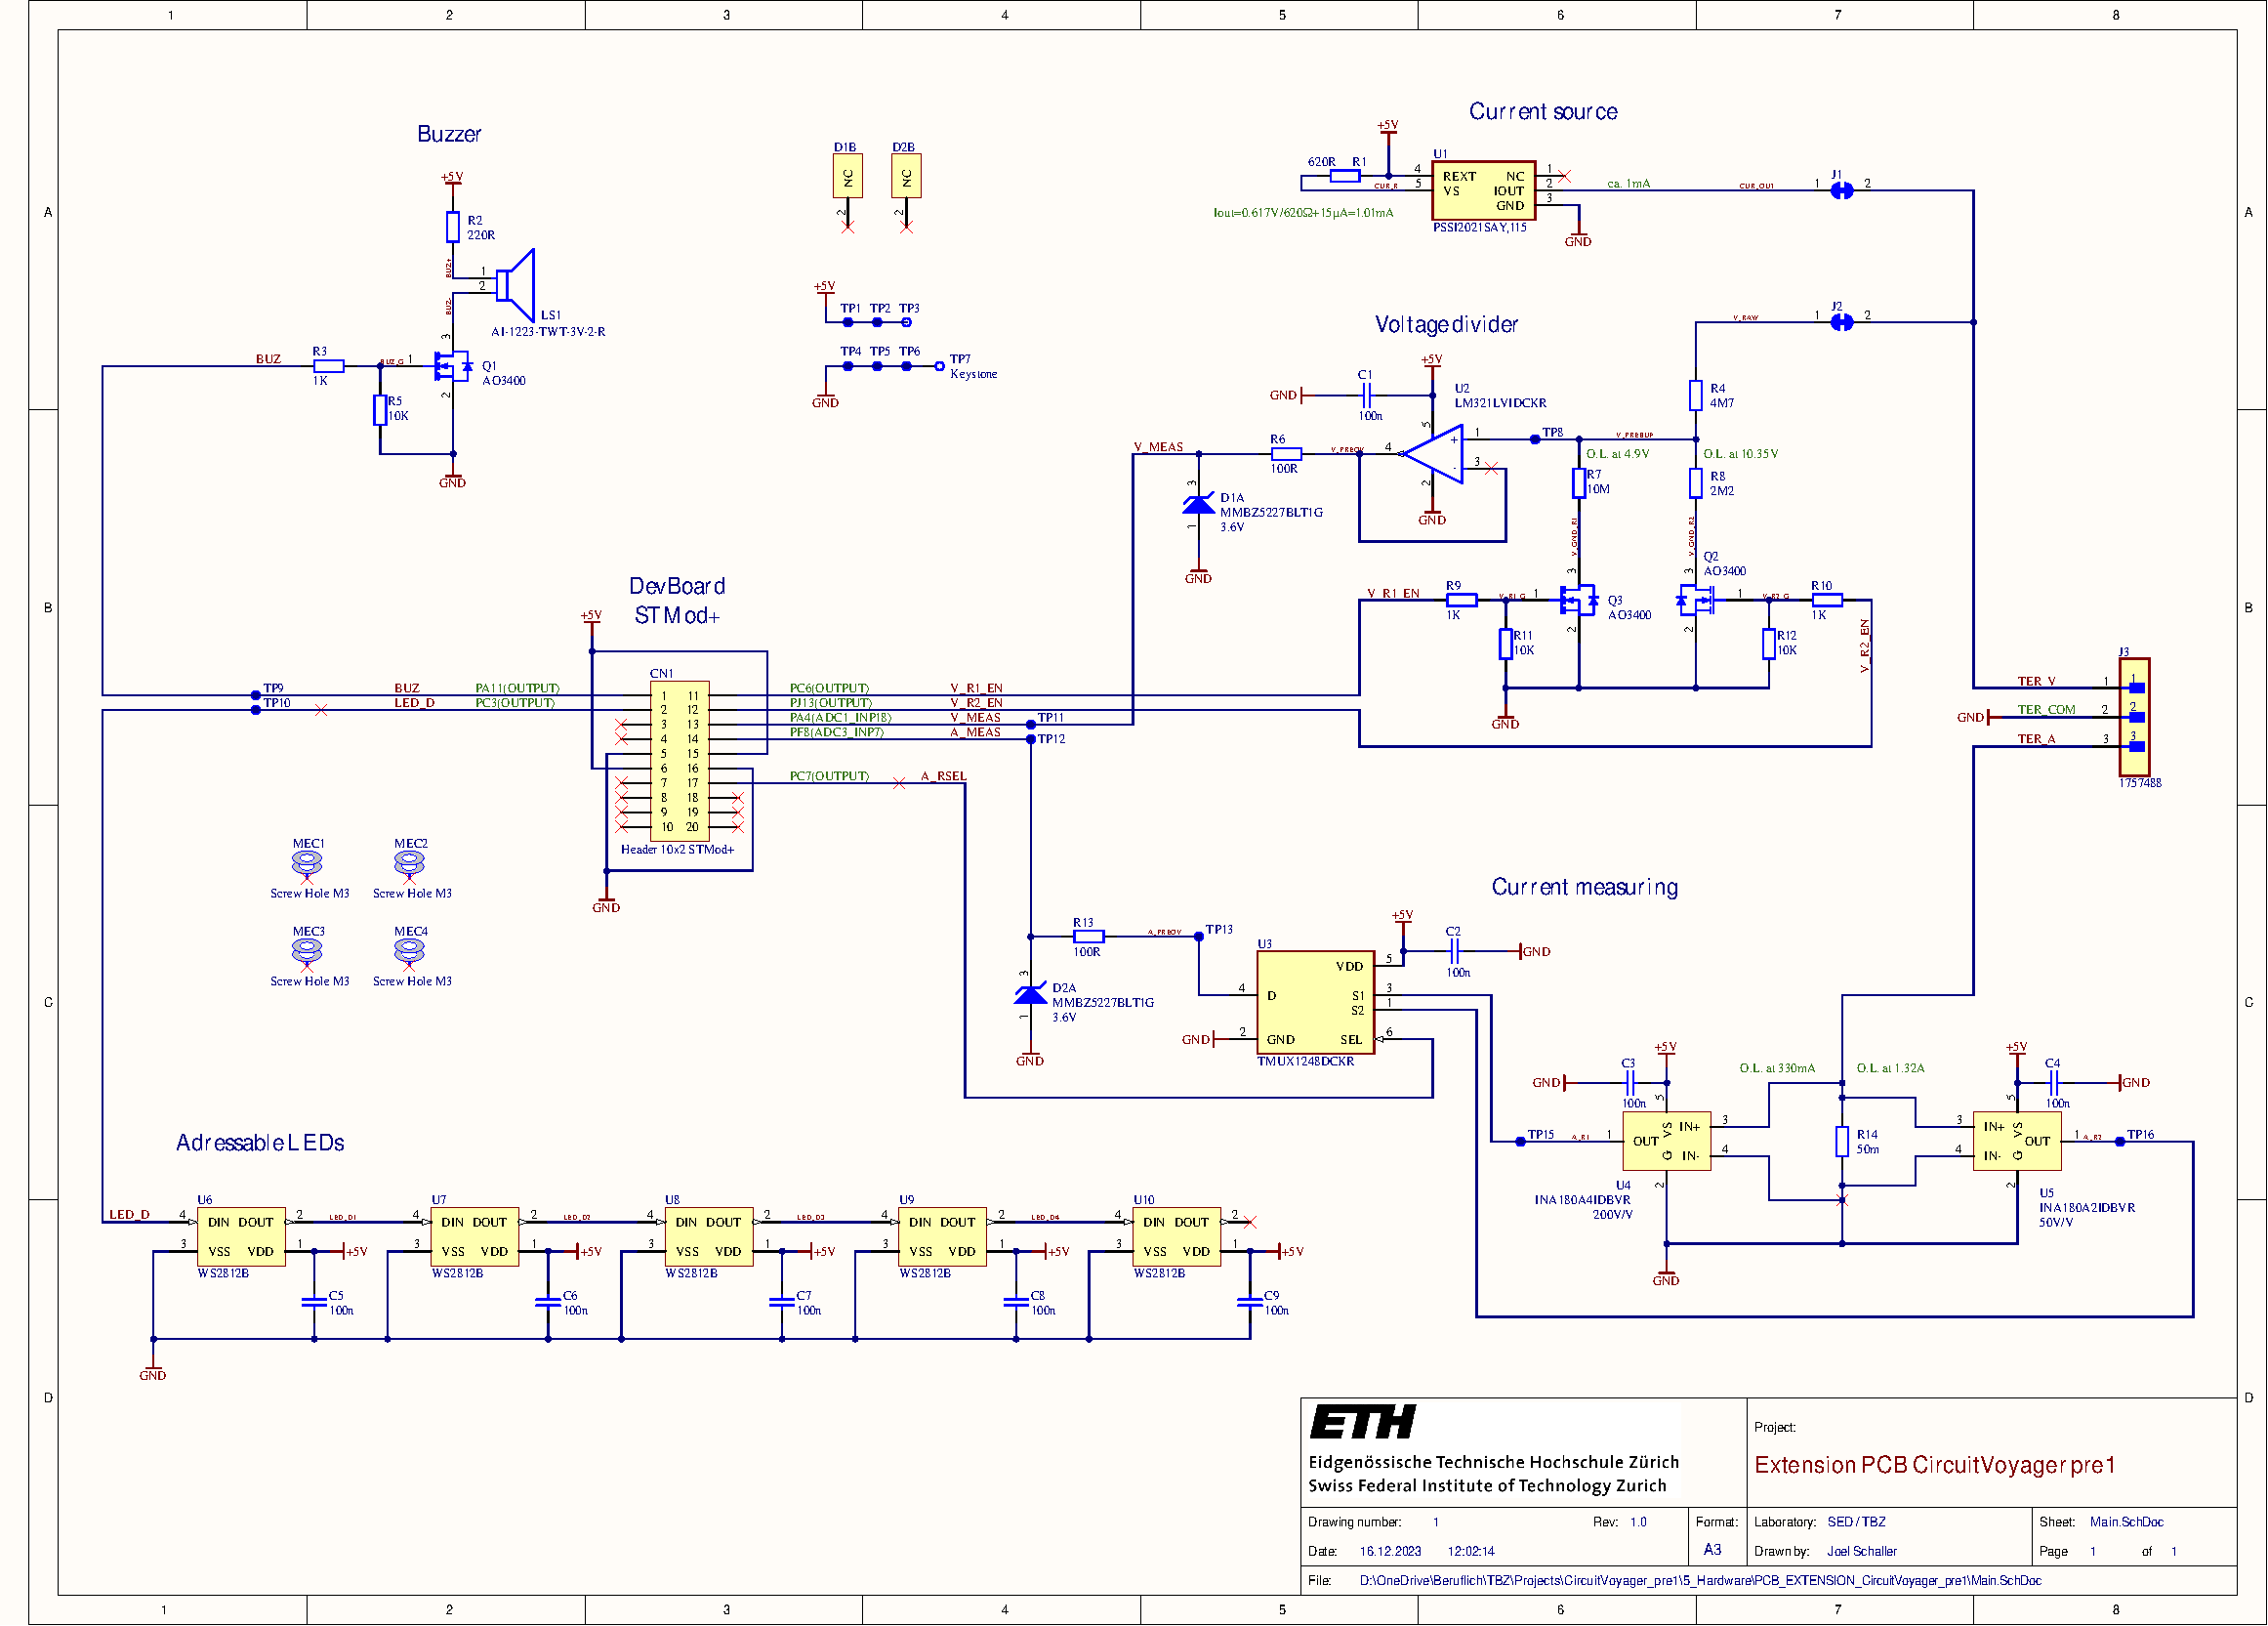
\includegraphics[width=8cm, trim={3.4cm 19cm 28.5cm 2cm}, clip]{../../../5_Hardware/PCB_EXTENSION_CircuitVoyager_pre1/Project Outputs for PCB_EXT_CV_PRE1/Schematic_PCB_EXTENSION_CircuitVoyager_pre1.pdf}
	\caption{Buzzer Circuit}
	\label{fig:Buzzer Circuit}
\end{figure}

This is an active buzzer. If the BUZ line is pulled high by the MCU, the MOSFET starts to conduct and the buzzer starts beeping. This circuit will be used to give an acoustic feedback to the user, if for example a continuity has been detected. 

The resistors R3 and R5 build a voltage divider with a ratio of 1/10. This has the advantage, that the gate capacitance of Q1 is charged with a limited current and if nothing's connected to the BUZ net, the MOSFET turns the buzzer off and the whole machine isn't in an indeterminate state.

The resistor R2 limit the current flowing through LS1. As LS1 is rated for 30mA at 3V.
\[R_2=\frac{U_{VCC}-U_{LS1}}{I_{LS1}}=\frac{5V-3V}{30mA}= \underline{\underline{66.\overline{6}\Omega}}\]

\[P_{R2}=I^2 \cdot R=(30mA)^2 \cdot 66. \overline{6} \Omega = \underline{\underline{60mW}}\]
Finally, I've chosen a 220\(\Omega\) resistor for R2. With this value the sound should be loud enough, that the user hears it. And the power loss of the resistor will be smaller. That means it should be perfectly fine to use a 0402 resistor that is rated for 62.5mW.


\subsubsection{Adressable LEDs Circuit}

\begin{figure}[H]
	\centering
	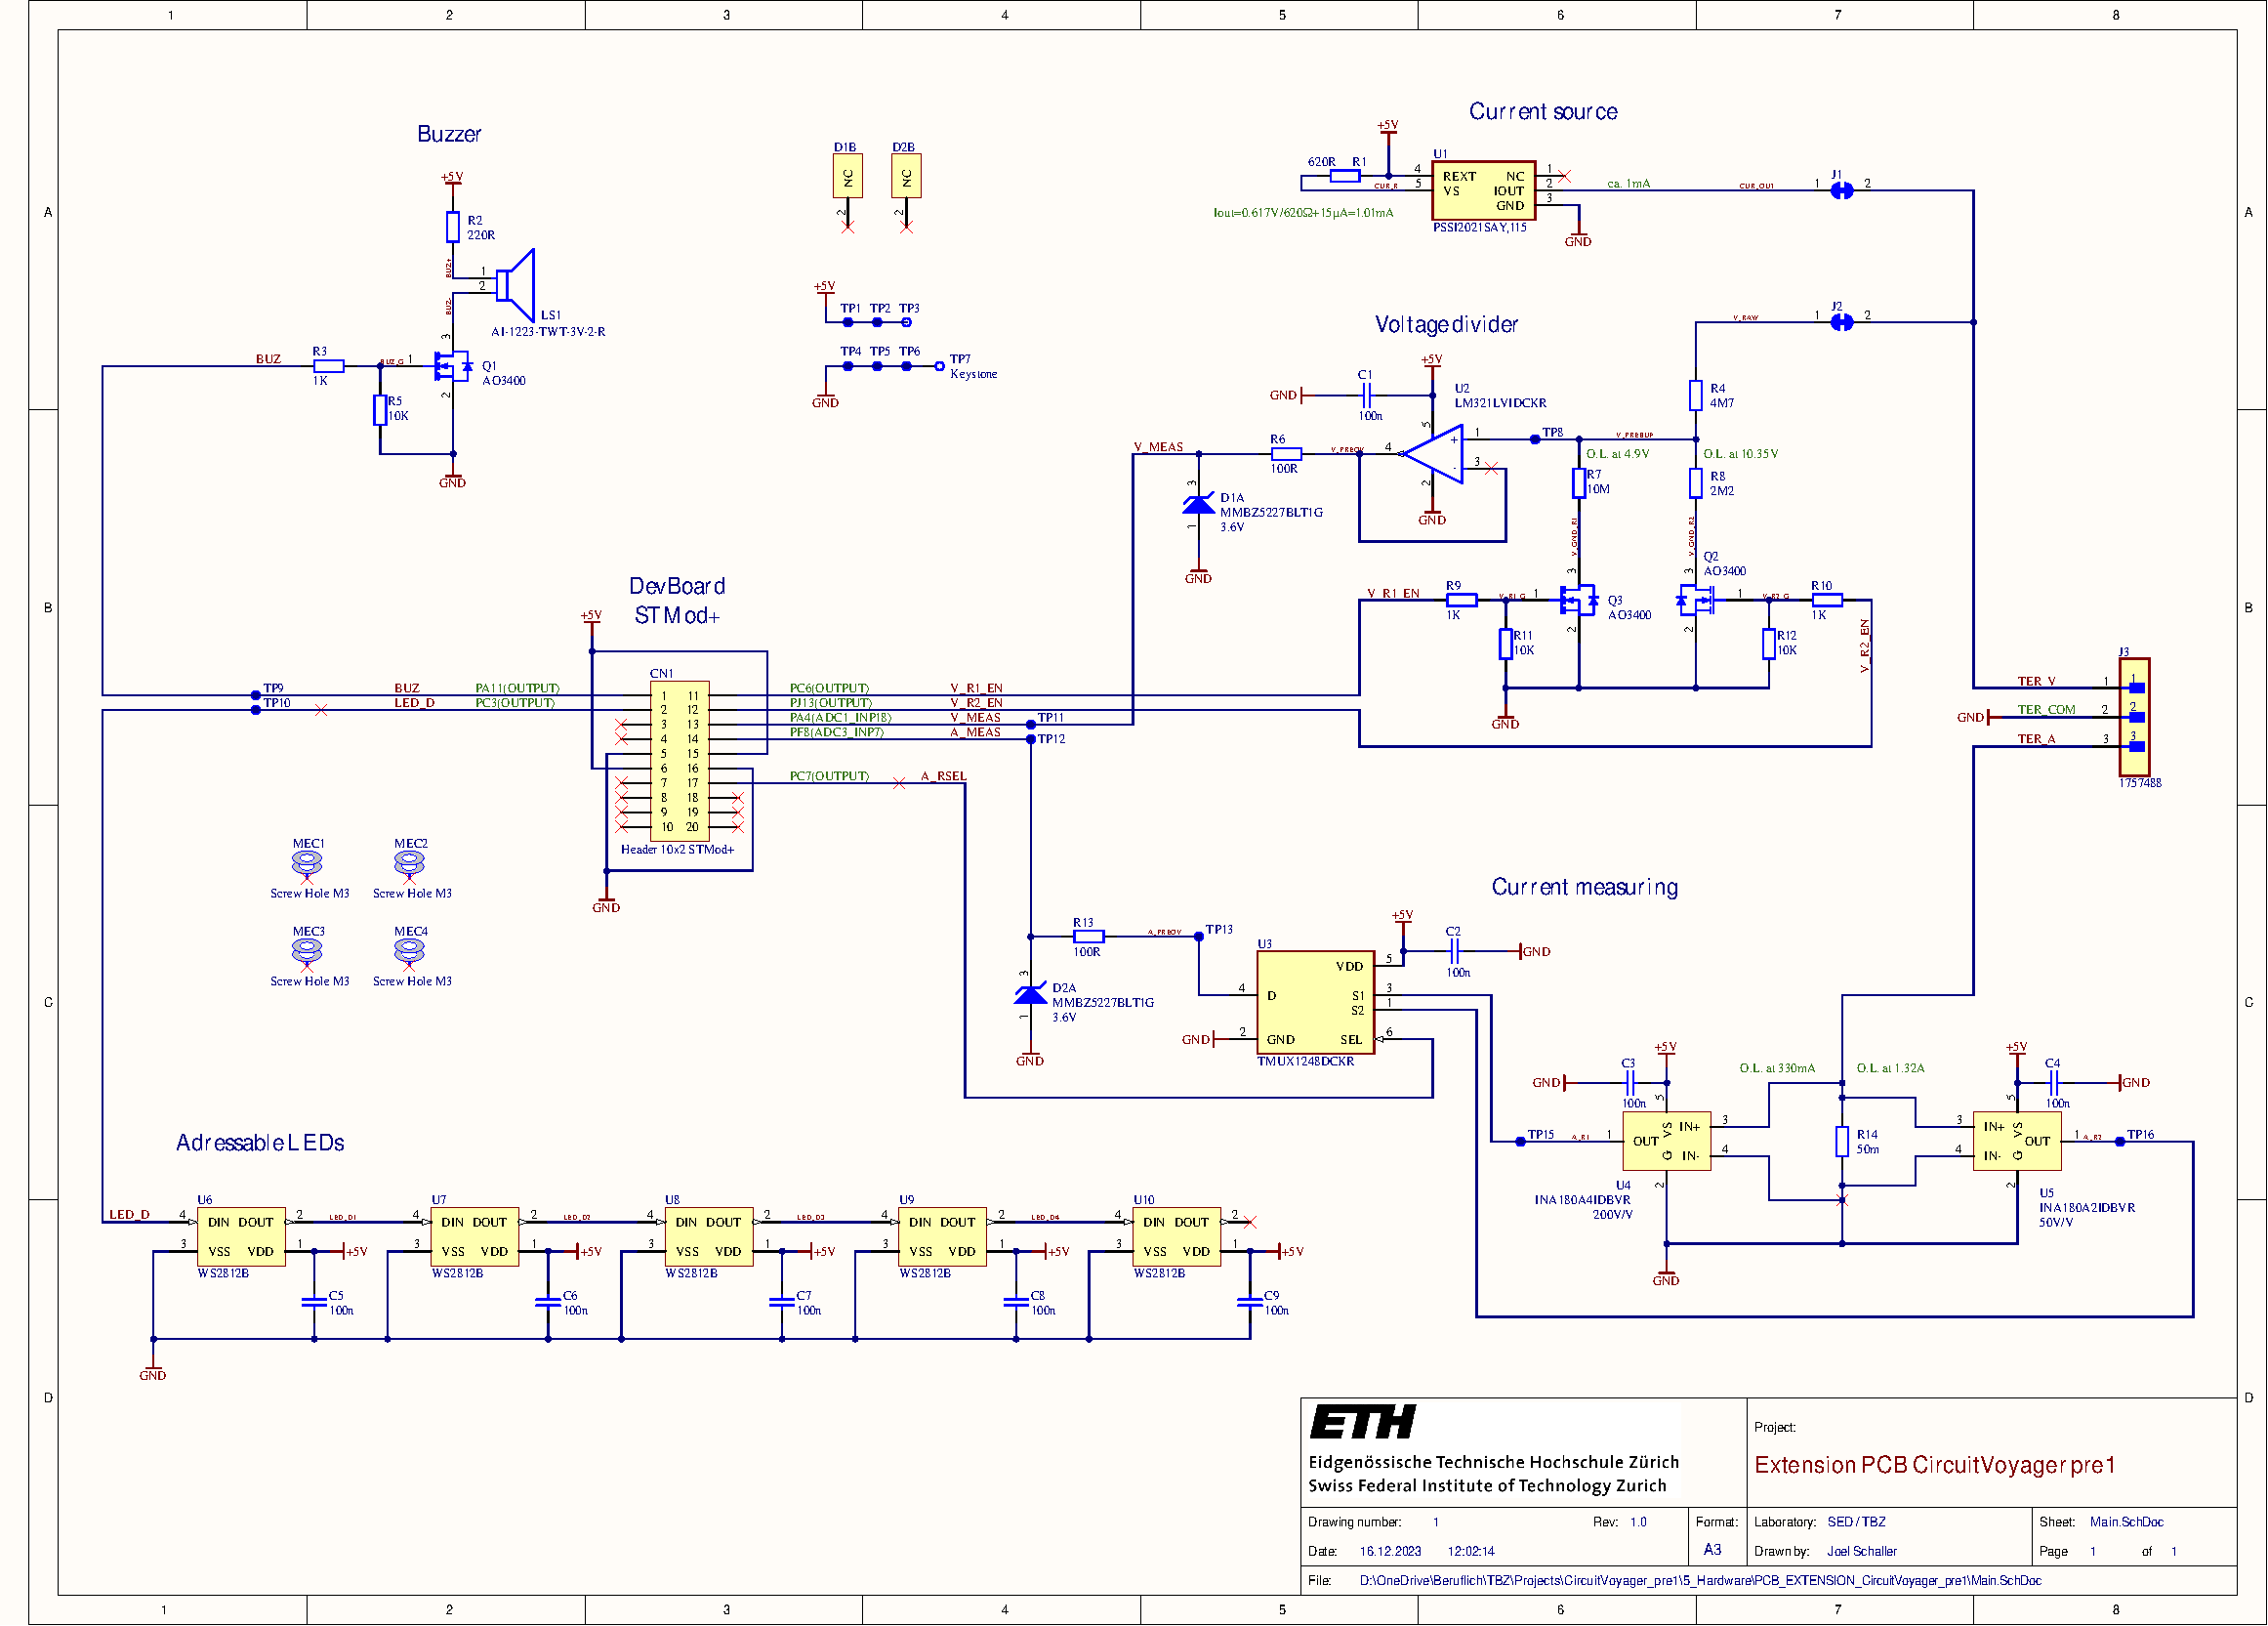
\includegraphics[width=15cm, trim={1.3cm 4cm 16.3cm 20cm}, clip]{../../../5_Hardware/PCB_EXTENSION_CircuitVoyager_pre1/Project Outputs for PCB_EXT_CV_PRE1/Schematic_PCB_EXTENSION_CircuitVoyager_pre1.pdf}
	\caption{Adressable LEDs Circuit}
	\label{fig:Adressable LEDs Circuit}
\end{figure}

An other option to show if continuity has been detected are these LEDs. The advantage of them is, that they only need one data connection and already include their logic and driving circuits. I've equiped them with one bulk capacitor each, because they're integrated components. They're driven over the 5V rail, which they're specified for. But if they're driven by 5V they theoretically detect all voltages over 3.5V as a logical high. But the MCU only outputs 3.3V. I've used those LEDs much in past projects and this was never a problem, so I'm assuming that it should also work this time.



\subsubsection{Overvoltage Protection Circuit}

\begin{figure}[H]
	\centering
	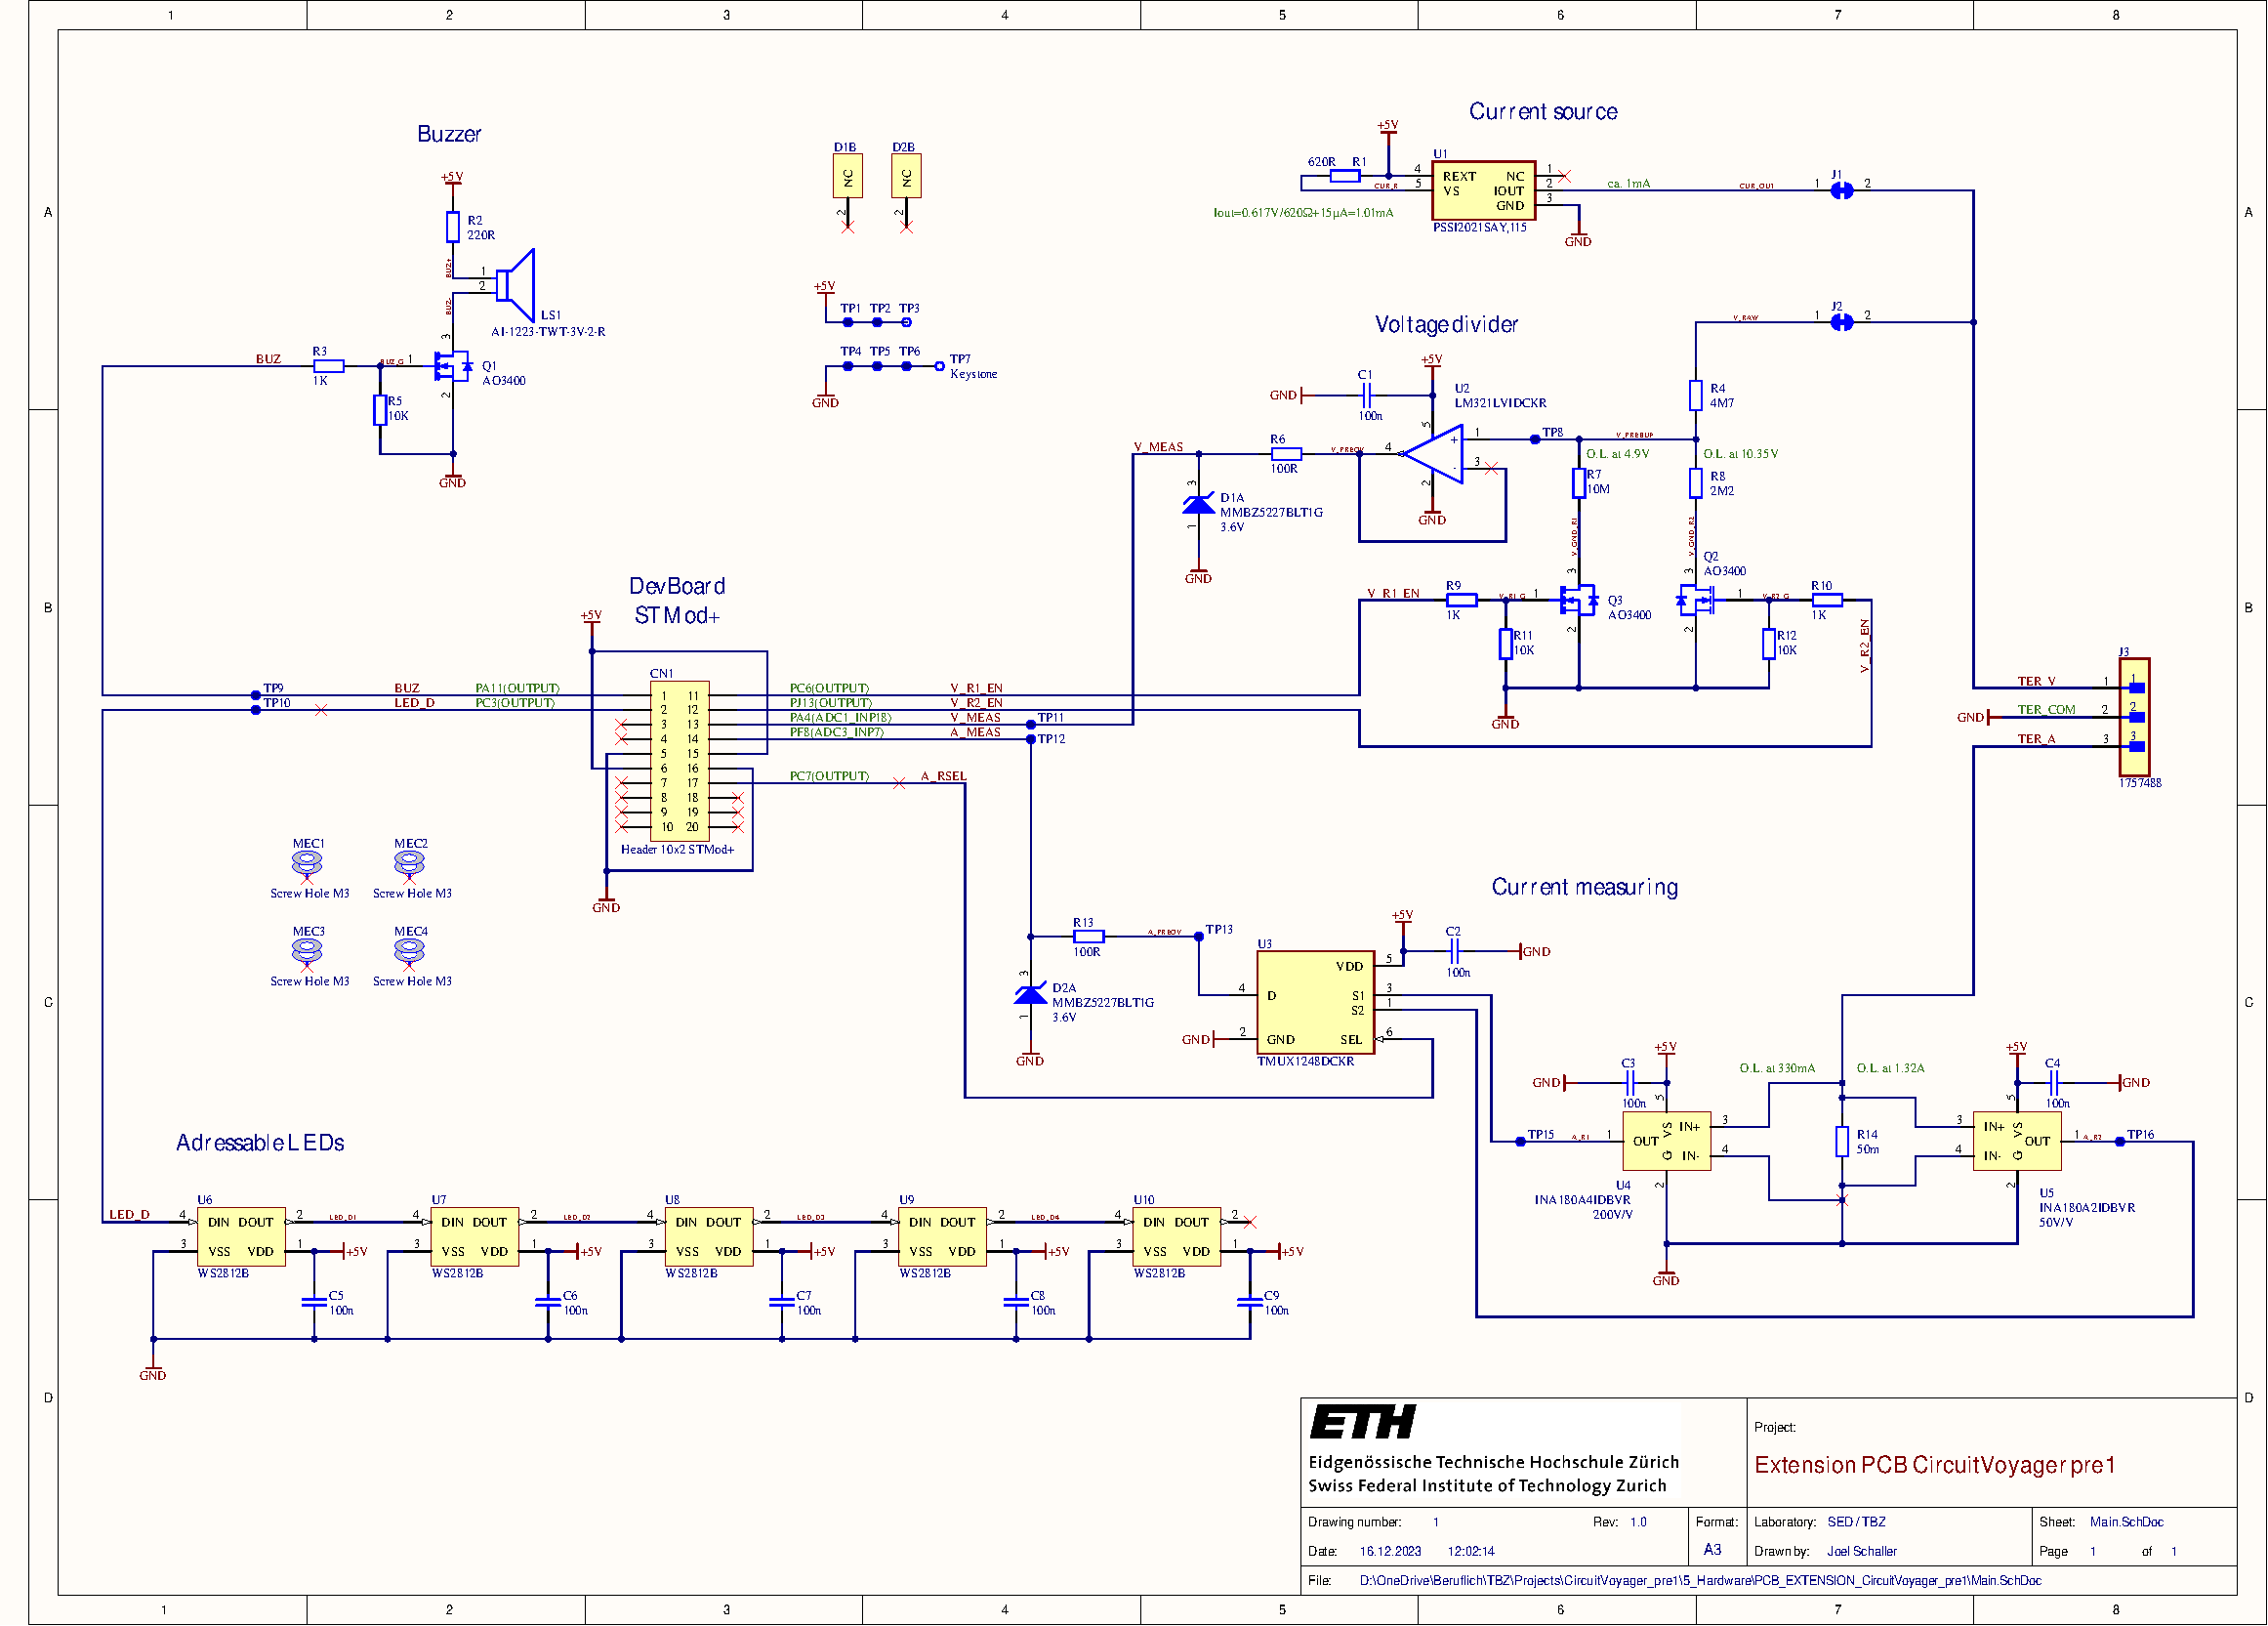
\includegraphics[width=6cm, trim={17cm 9.5cm 19cm 15.5cm}, clip]{../../../5_Hardware/PCB_EXTENSION_CircuitVoyager_pre1/Project Outputs for PCB_EXT_CV_PRE1/Schematic_PCB_EXTENSION_CircuitVoyager_pre1.pdf}
	\caption{Overvoltage Protection Circuit}
	\label{fig:Overvoltage Protection Circuit}
\end{figure}

My Problem is, that the voltages coming from  the extension PCB, can't exceed 4V according to the MCUs datasheet. But because this PCB is powered by the 5V rail, theoretically these voltages could damage the MCU. So the goal was to develop a circuit which protects the ADC inputs. The first idea that came to my mind was to use varistors. I've already used them once in a project, but after reading some application notes on this topic, I decided to use a zenerdiode for the OVP. \cite{Protecting_ADC_Inputs_AN}

The zenerdiode I've used has a nominal zenervoltage of 3.6V (max. 3.78V) at 20mA. Together with R13 this should result in a maximum voltage of 3.78V at the ADC inputs. As long as the PREOV voltage doesn't exceed 5.6V.
\[U_{PREOV(MAX.)} = R_{13} \cdot I_Z + U_Z = 100\Omega \cdot 20mA + 3.6V = \underline{\underline{5.6V}}\]
\[P_{R13} = R \cdot I^2 = 100\Omega \cdot (20mA)^2 = \underline{\underline{40mW}}\]


\subsubsection{Voltage Divider Circuit}

\begin{figure}[H]
	\centering
	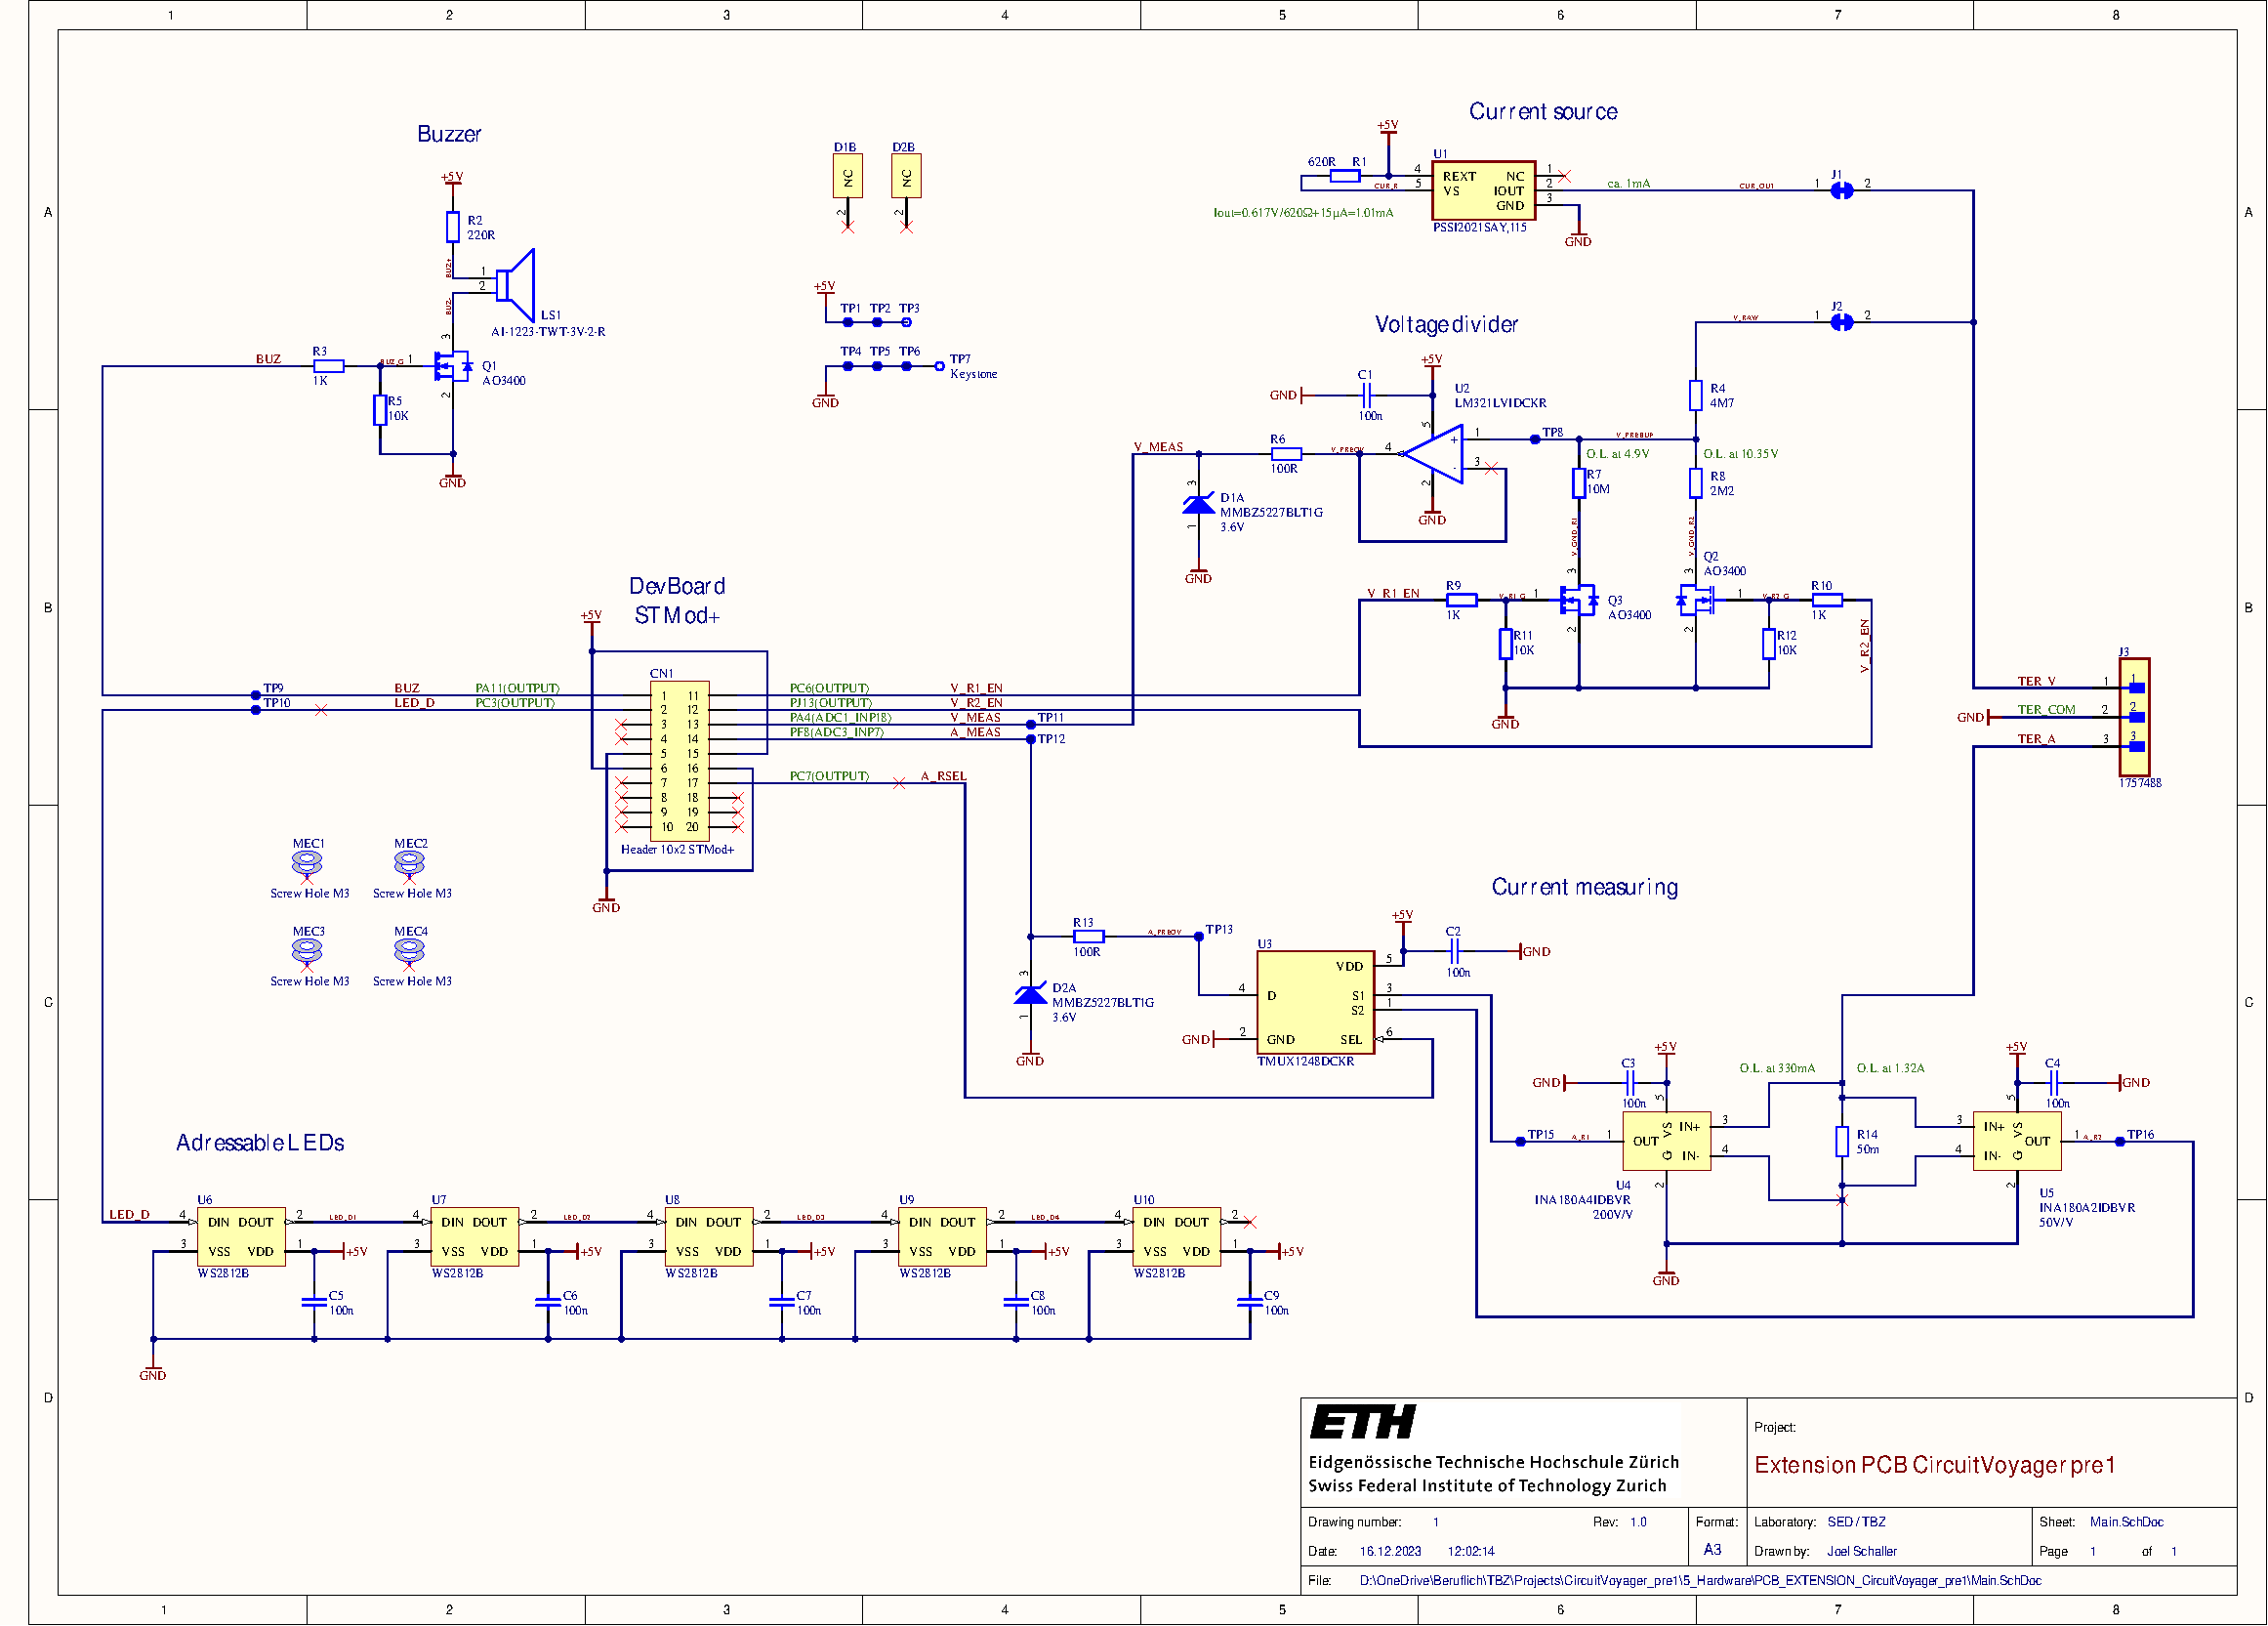
\includegraphics[width=12cm, trim={23cm 15cm 6cm 5cm}, clip]{../../../5_Hardware/PCB_EXTENSION_CircuitVoyager_pre1/Project Outputs for PCB_EXT_CV_PRE1/Schematic_PCB_EXTENSION_CircuitVoyager_pre1.pdf}
	\caption{Voltage Divider Circuit}
	\label{fig:Voltage Divider Circuit}
\end{figure}

The voltage divider is used to measure voltages over the V terminal. This circuit is one approach to range switching, which is described more detailed in the following chapter [\ref{subsec:rangeswitching}]. This voltage divider features 2 ranges and I came up with this idea by myself. The ranges are calculated as following:
\[U_{OL(R1)} = \frac{(R_4 + R_7) \cdot U_{OL(MCU)}}{R_7} = \frac{(4.7M\Omega + 10M\Omega) \cdot 3.3V}{10M\Omega} = \underline{\underline{4.851V}}\]
\[U_{OL(R2)} = \frac{(R_4 + R_8) \cdot U_{OL(MCU)}}{R_8} = \frac{(4.7M\Omega + 2.2M\Omega) \cdot 3.3V}{2.2M\Omega} = \underline{\underline{10.35V}}\]
This divided voltage is then fed into an impedance converter which guarantees that the voltage divider isn't manipulated by the ADCs internal resistance and also helps on the DevBoards analog paths, because they're very long and therefore vulnerable to electromagnetic fields.



\subsubsection{Current Source Circuit}

\begin{figure}[H]
	\centering
	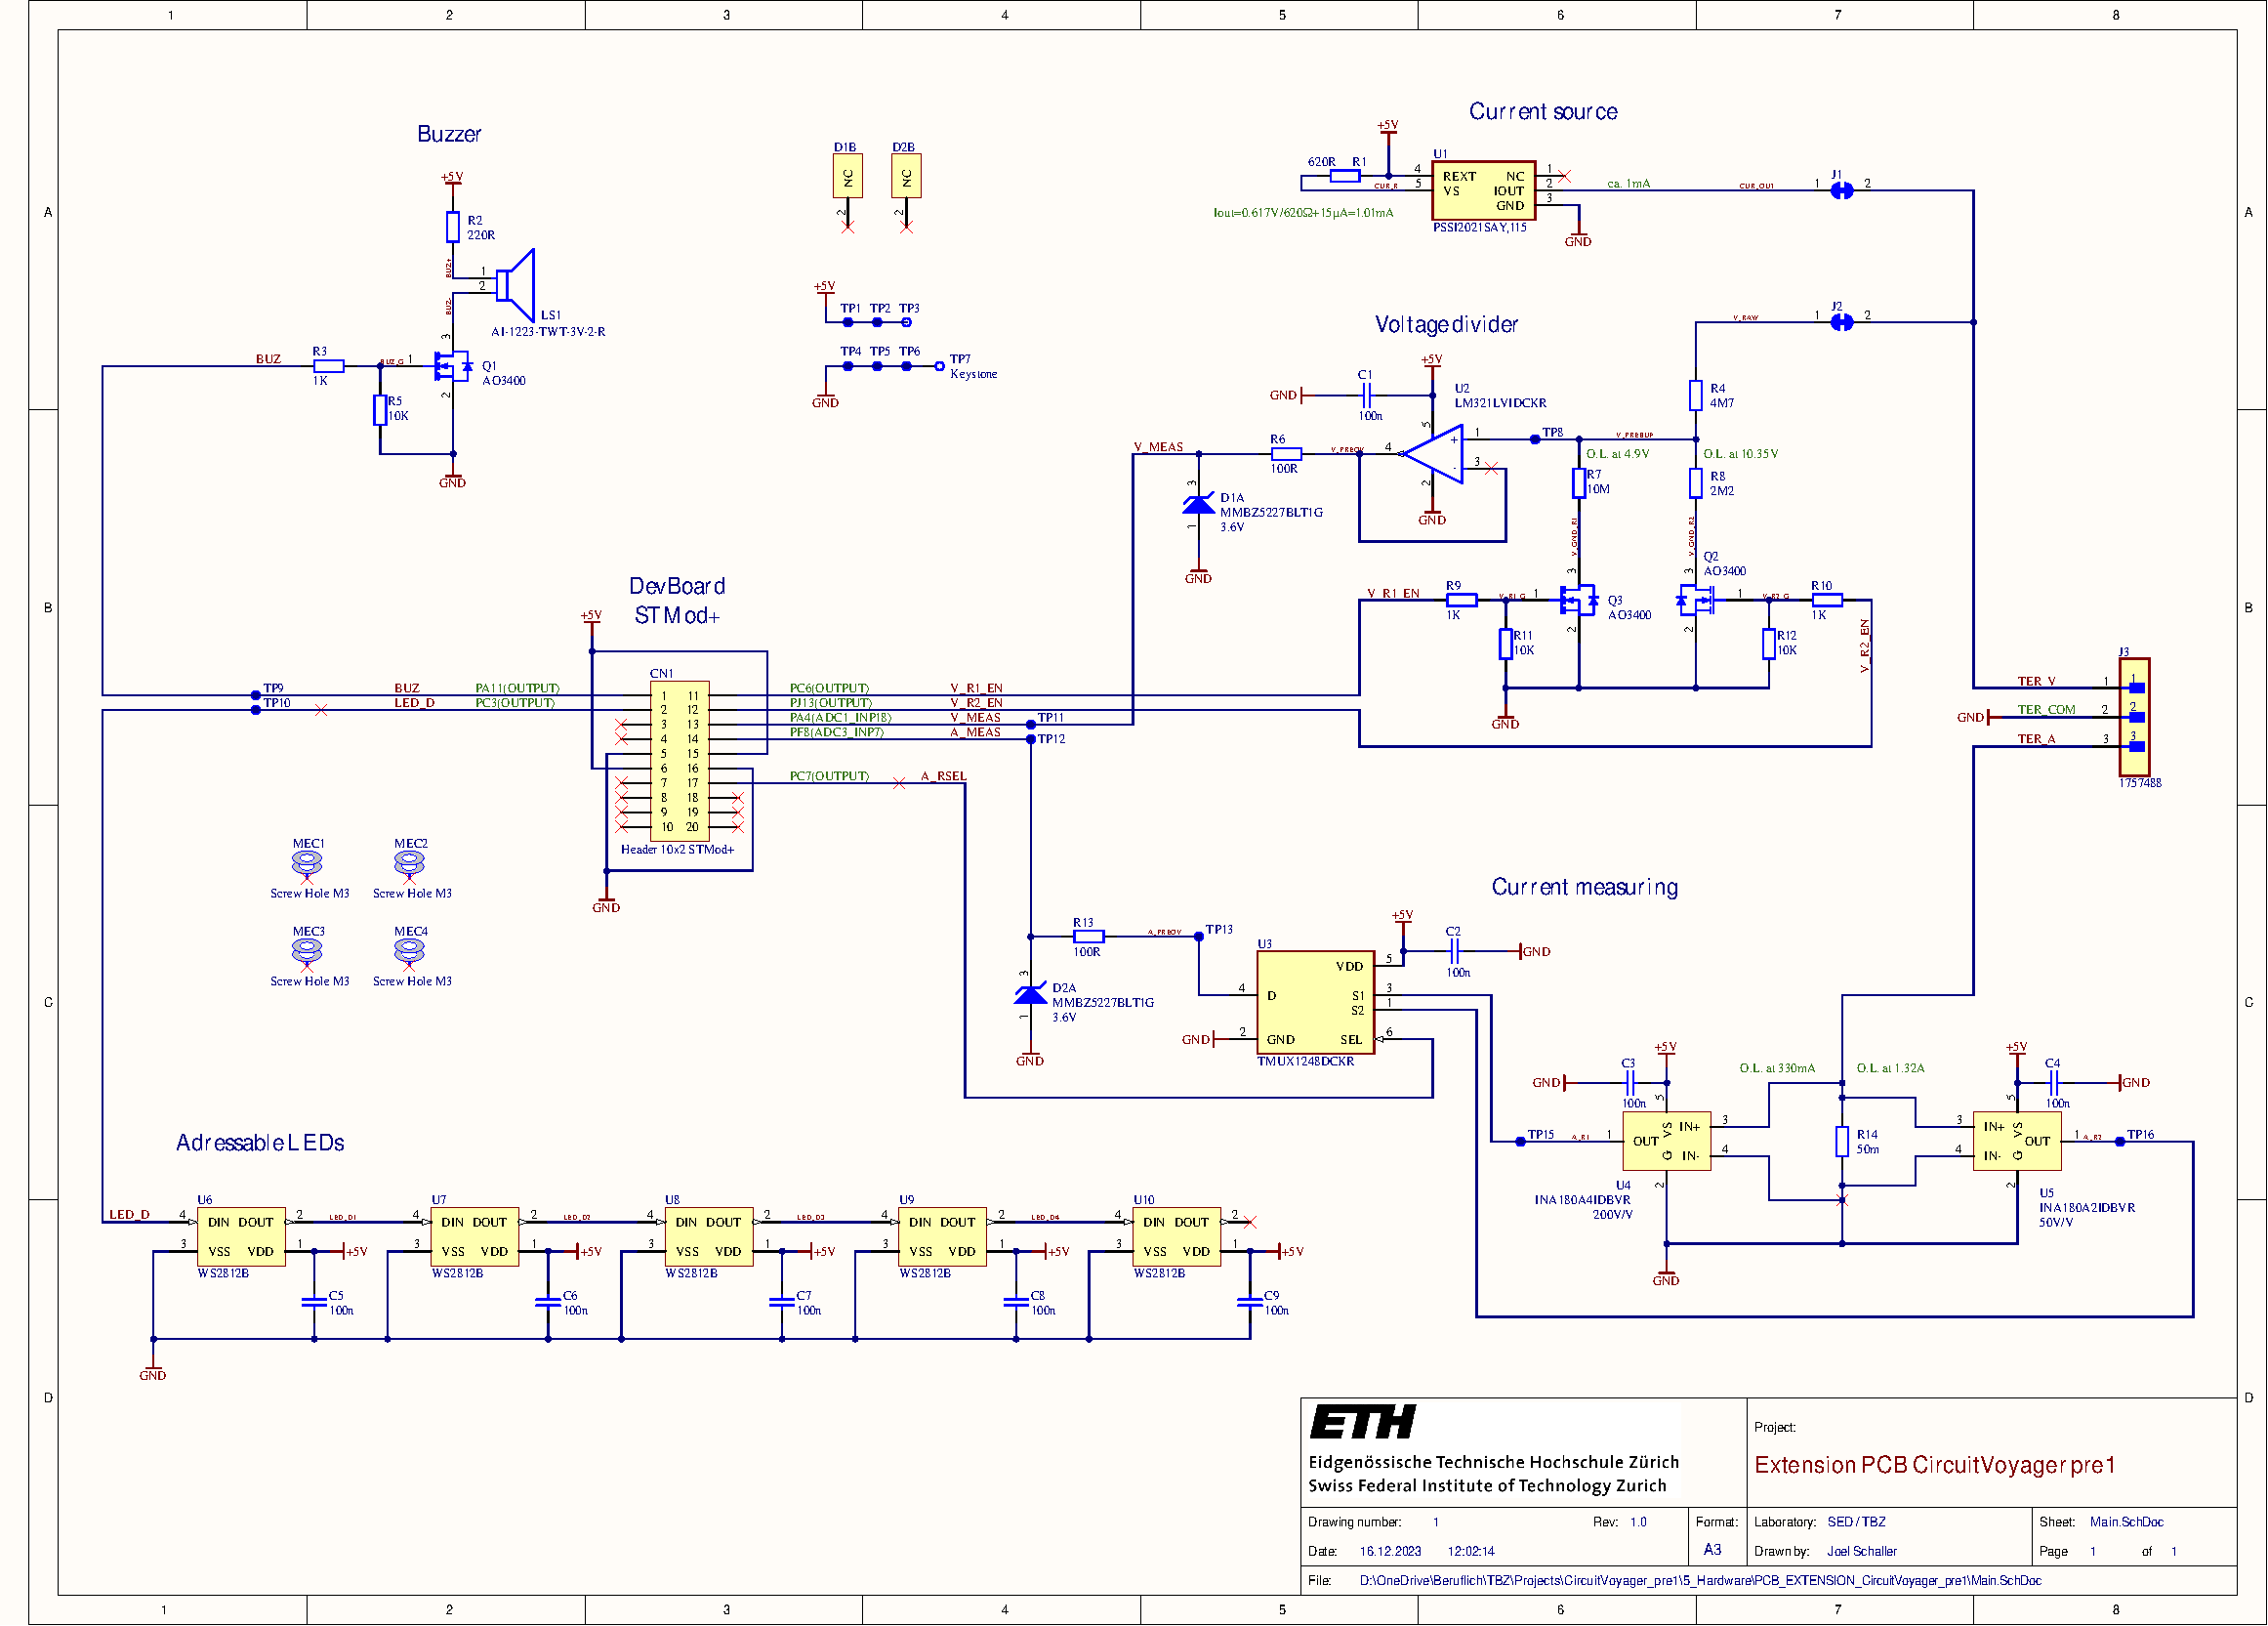
\includegraphics[width=10cm, trim={20cm 23cm 10cm 1cm}, clip]{../../../5_Hardware/PCB_EXTENSION_CircuitVoyager_pre1/Project Outputs for PCB_EXT_CV_PRE1/Schematic_PCB_EXTENSION_CircuitVoyager_pre1.pdf}
	\caption{Current Source Circuit}
	\label{fig:Current Source Circuit}
\end{figure}

The current source circuit will be used to measure continuity and resistance, together with the voltage measuring function. A constant current will be induced to the DUT and because the voltage over the DUT can be measured, the resistance can be calculated. The constant current can be calculated as following:
\[I_{OUT} = \frac{U_{VS}}{R_1} + 15\mu A = \frac{0.617V}{620\Omega} + 15\mu A = \underline{\underline{1.01mA}}\]
But this doesn't matter that much, because the DMM will be calibrated using the solderbridge J1.
\\
\todo[inline, color=red!40]{Note that this circuit isn't used in the final design, because there's no option to disconnect this circuit from the voltage measuring circuit via the MCU. So I decided to leave the current source disconnected from the rest of the circuits. More information in chapter [\ref{sssec:baddesign}].}



\subsubsection{Current Measuring Circuit}

\begin{figure}[H]
	\centering
	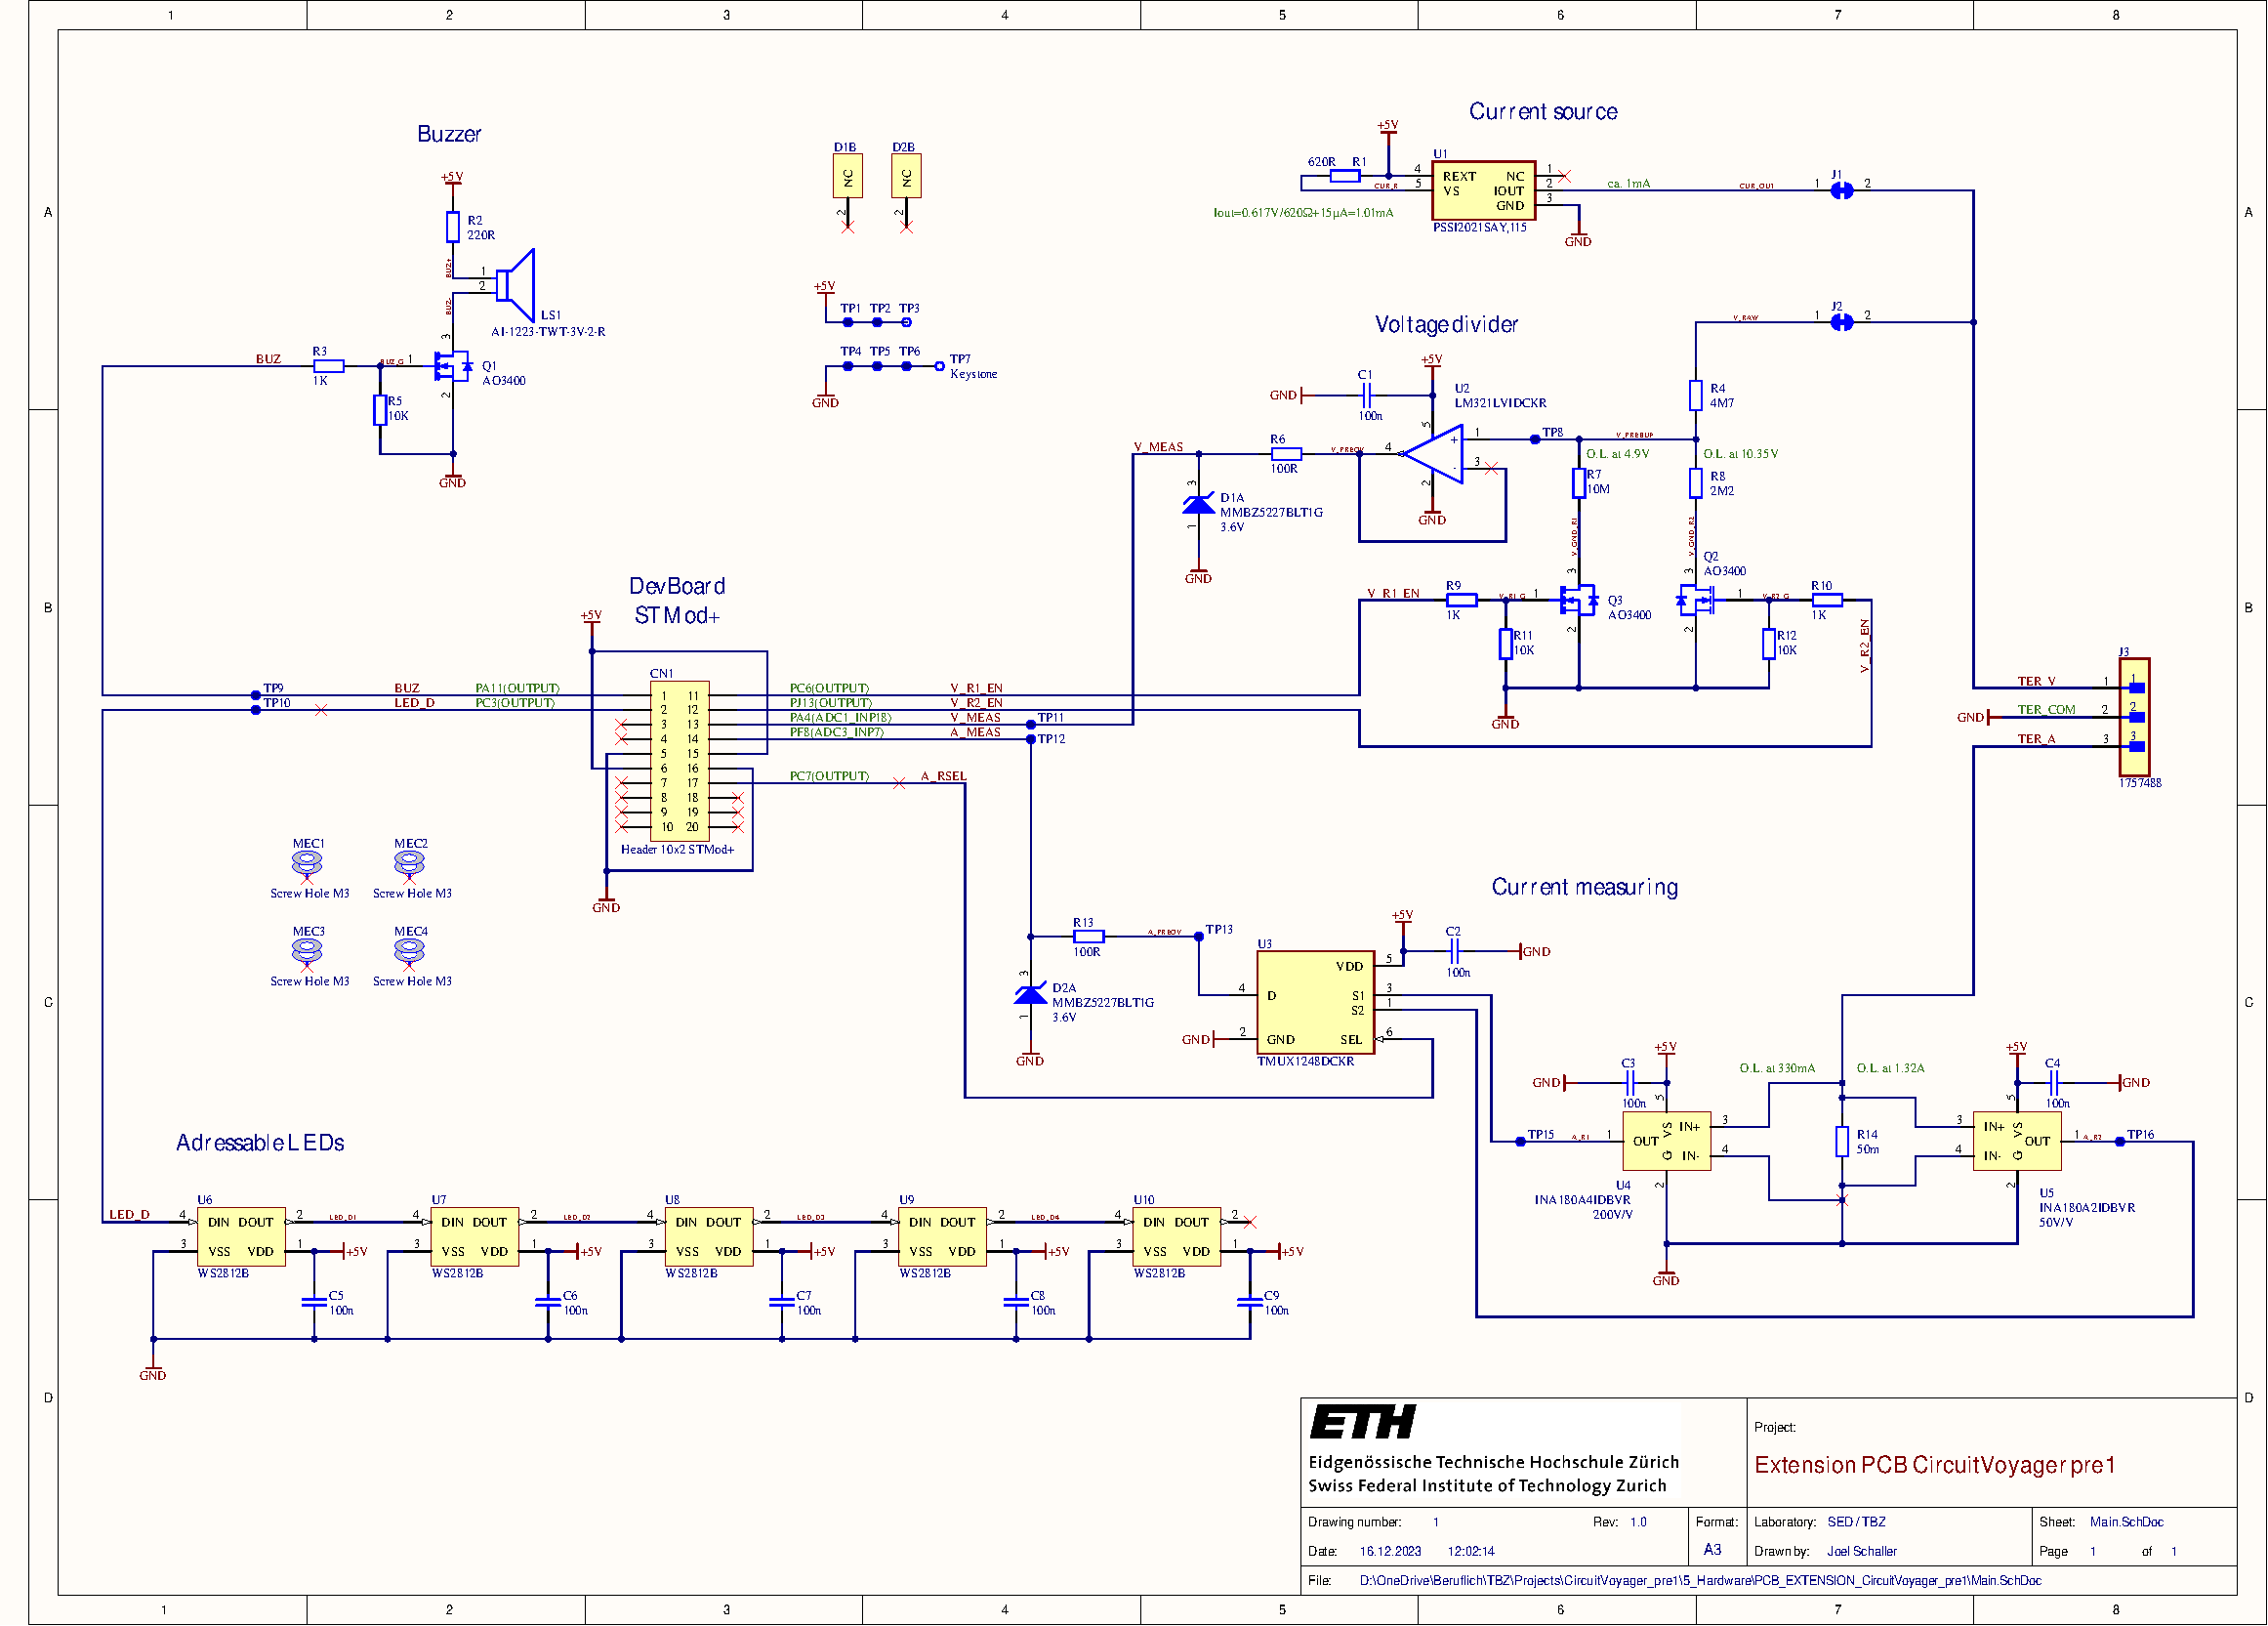
\includegraphics[width=14cm, trim={19.5cm 5cm 1cm 14.5cm}, clip]{../../../5_Hardware/PCB_EXTENSION_CircuitVoyager_pre1/Project Outputs for PCB_EXT_CV_PRE1/Schematic_PCB_EXTENSION_CircuitVoyager_pre1.pdf}
	\caption{Current Measuring Circuit}
	\label{fig:Current Measuring Circuit}
\end{figure}

The current measuring circuit is used to measure currents with the A terminal. This circuit is one approach to range switching, which is described more detailed in the following chapter [\ref{subsec:rangeswitching}]. This circuit features 2 ranges and I came up with this idea, while reading some articles on DMMs \cite{Digital_multimeter_circuit_using_ICL7107} \cite{AN-202_A_Digital_Multimeter_Using_the_ADD3501}. The ranges are calculated as following:
\[I_{OL(R1)} = \frac{U_{OL(MCU)}}{R_{14} \cdot G_{U4}} = \frac{3.3V}{50m\Omega \cdot 200\frac{V}{V}} = \underline{\underline{330mA}}\]
\[I_{OL(R2)} = \frac{U_{OL(MCU)}}{R_{14} \cdot G_{U5}} = \frac{3.3V}{50m\Omega \cdot 50\frac{V}{V}} = \underline{\underline{1.32A}}\]
These voltages are then fed into an analog MUX, which switches the processed voltages to the ADC. This has the advantage, that the DMM doesn't manipulate the actual path, where the current is flowing through and therefore not influencing the DUT.

The power rating of R14 is 125mW, while the maximal power loss of R14 at 1.32A is 87.12mW.
\[P_{R14} = I^2 \cdot R = (1.32A)^2 \cdot 50m \Omega = \underline{\underline{87.12mW}}\]



\newpage
\subsection{PCB}
\subsubsection{Layout}

The PCB layout was also made in Altium Designer. This was therefore also my first layout in Altium Designer. The only problem I had, were the vias. I had to improvise by setting their parameters manually instead of letting Altium do it. 

\begin{figure}[H]
	\centering
	\includegraphics[width=5.5cm, page=2]{Resources/PCB_LAyout.png}
	\caption{Extension PCB Layout}
	\label{fig:Extension PCB Layout}
\end{figure}

Later I've generated the output files (Gerber files, BOM, assembly drawing) and ordered the PCB on JLCPCB with 2 layers, tented vias, removed order number and blue solder mask. The BOM is in the appendix chapter [\ref{sec:Extension PCB Manufacture 11.23 BOM}]. The components were sourced using DigiKey and ETH SPH.

\subsubsection{Assembly}

Then I've assembled the PCB by hand, which wasn't a problem at all. But it turned out, that I've ordered the wrong connectors for the STMod interface. Instead of the 4mm long pins I've ordered the 2mm long pins, which don't make contact with the socket from the DevBoard. But luckily I was able to order longer ones, which arrived quite fast.

\begin{figure}[H]
	\centering
	\includegraphics[height=10cm, page=2]{../../../5_Hardware/PCB_EXTENSION_CircuitVoyager_pre1/Project Outputs for PCB_EXT_CV_PRE1/PCB_EXTENSION_CircuitVoyager_pre1.pdf}
	\caption{Extension PCB Assembly Drawing}
	\label{fig:Extension PCB Assembly Drawing}
\end{figure}



\begin{figure}[H]
	\centering
	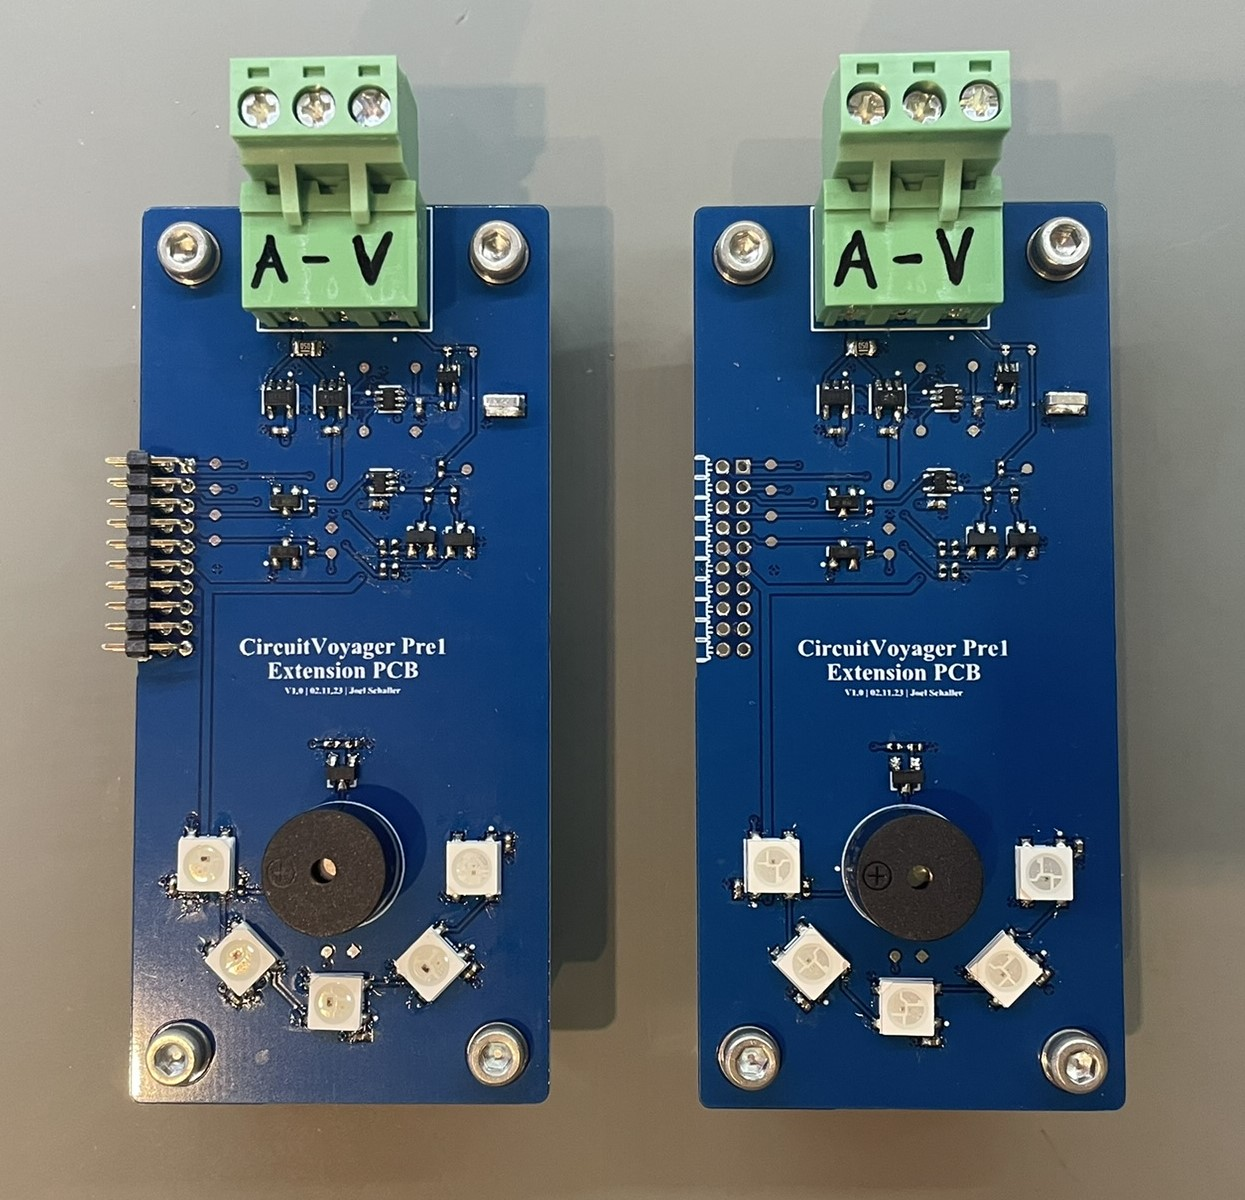
\includegraphics[height=10cm]{Resources/PCB.png}
	\caption{Extension PCB}
	\label{fig:Extension PCB}
\end{figure}

\newpage
\subsubsection{Commissioning}
\label{subsec:commissioning}
I've only documented one commissioning of the 2 PCBs. The other one was tested, using the same process.

\begin{table}[H]
	\centering
	\label{tab:commissioning PCB 1}
\begin{tabular}{|| c | c | c | c ||} 
\hline
Action & Measurement point & Expected & Measured \\ [0.5ex] 
\hline\hline
Connect power supply @ 5V & CN1.6 \(\rightarrow\) TP7 & max. 100mA & \textcolor{Green}{\textbf{18mA}} \\
\hline
Test Buzzer (TP9 to 3.3V) & acoustic & beeps & \textcolor{Green}{\textbf{PASS}} \\
\hline
Test const. Current & J3.1 & 1mA & \textcolor{Red}{\textbf{13mA}} \\
\hline
LEDs on with AWG (CN1.2) & optical & lights up & \textcolor{Green}{\textbf{PASS}} \\
\hline
Current meas. test Range 1 & CN1.14 & 10V/A & \textcolor{Green}{\textbf{fig: \ref{fig:Commissioning PCB1 current measurements}}} \\
\hline
Current meas. test Range 2 & CN1.14 & 2.5V/A & \textcolor{Green}{\textbf{fig: \ref{fig:Commissioning PCB1 current measurements}}} \\
\hline
Voltage meas. test Range 1 & CN1.13 & 0.68V/V & \textcolor{Green}{\textbf{fig: \ref{fig:Commissioning PCB1 voltage measurements}}} \\
\hline
Voltage meas. test Range 2 & CN1.13 & 0.32V/V & \textcolor{Green}{\textbf{fig: \ref{fig:Commissioning PCB1 voltage measurements}}} \\
\hline
\end{tabular}
	\caption{commissioning PCB 1}
\end{table}



\begin{figure}[H]
	\centering
	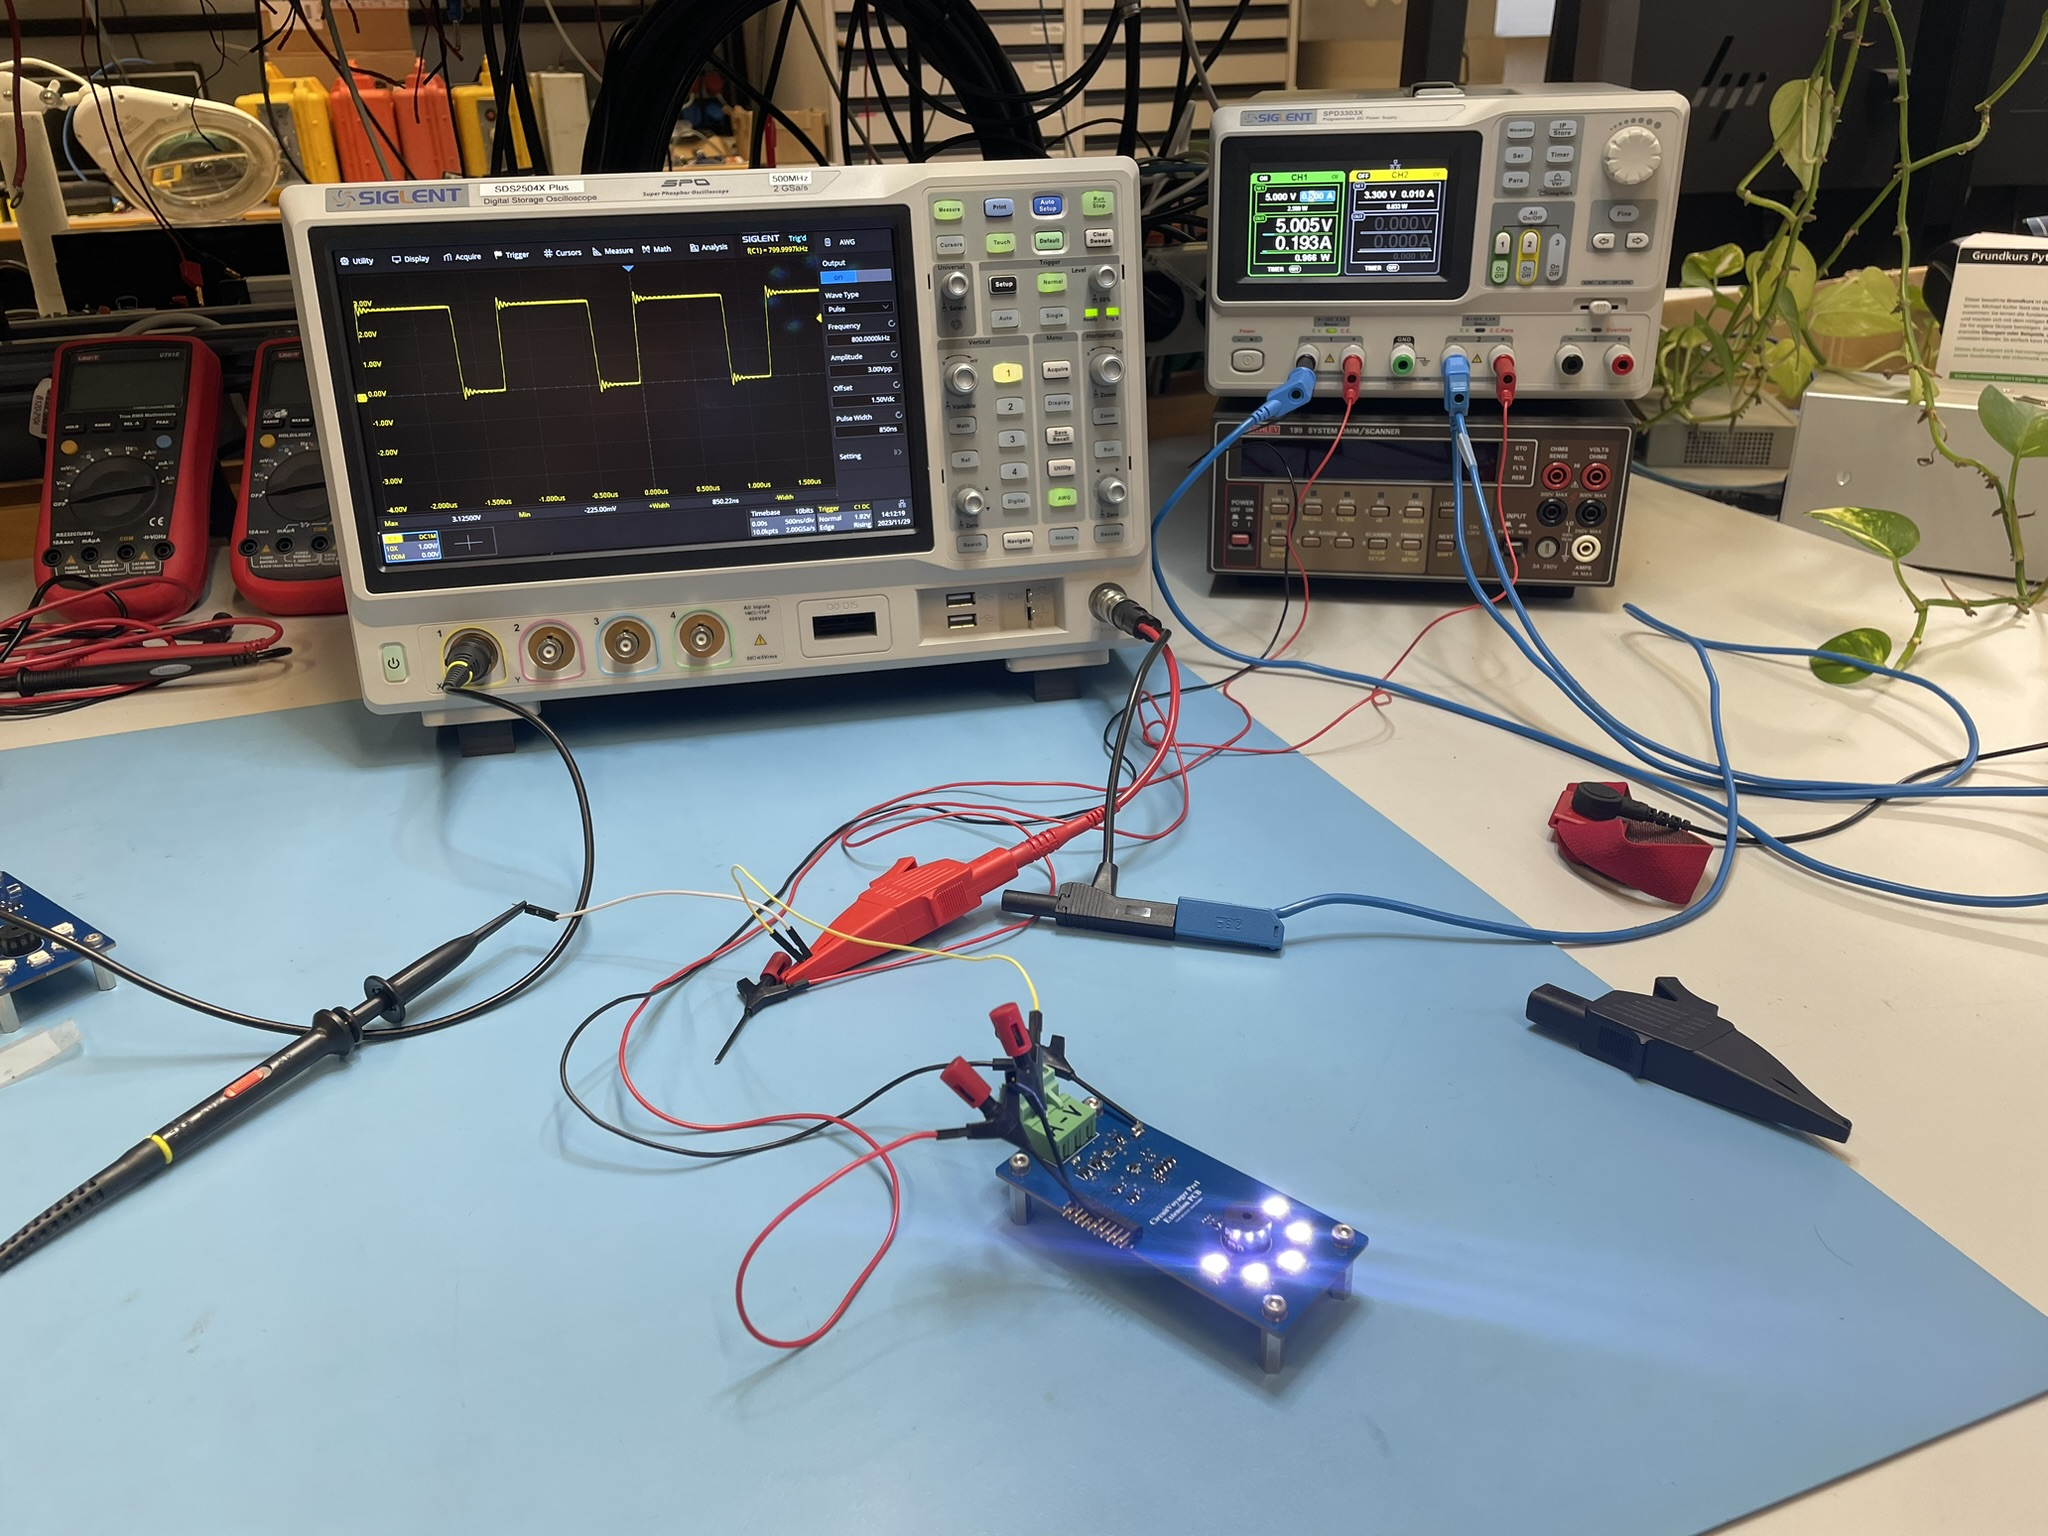
\includegraphics[width=15cm]{Resources/comissioning_lab_build.JPEG}
	\caption{Commissioning Lab}
	\label{fig:Commissioning Lab}
\end{figure}



\begin{figure}[H]
	\centering
	\begin{tikzpicture}
		\begin{groupplot}[
		group style={
			group size=1 by 2,
			horizontal sep=0cm,
			ylabels at=edge left,
		},
		width=13cm,
		height=3.5cm,
		scale only axis,
		xmin=0,xmax=1600,
		xtick distance=200,
		enlargelimits=false,
		grid=major,
		]
		
		\nextgroupplot[ylabel=$ U_{TP12(R1)} $, y unit=mV, xticklabels={}, ymin=0, ymax=3500, ytick distance=500]
		\addplot[red] coordinates { (1, 23) (5, 64) (10, 116) (50, 533) (100, 1050) (200, 2070) (400, 3320) (600, 3460) (800, 3480)};

		\nextgroupplot[ylabel=$ U_{TP12(R2)} $, y unit=mV, xlabel=$ I $,x unit=mA, ymin=0, ymax=3500, ytick distance=500]
		\addplot[ForestGreen] coordinates { (1, 7) (100, 273) (200, 544) (400, 1080) (600, 1620) (800, 2140) (1000, 2600) (1200, 2970) (1400, 3240) (1600, 3460)};
		
		\end{groupplot}
	\end{tikzpicture}
\caption{Commissioning PCB1 current measurements}
\label{fig:Commissioning PCB1 current measurements}
\end{figure}








\begin{figure}[H]
	\centering
	\begin{tikzpicture}
		\begin{groupplot}[
		group style={
			group size=1 by 2,
			horizontal sep=0cm,
			ylabels at=edge left,
		},
		width=13cm,
		height=3.5cm,
		scale only axis,
		xmin=0,xmax=16,
		xtick distance=2,
		enlargelimits=false,
		grid=major,
		]
		
		\nextgroupplot[ylabel=$ U_{TP11(R1)} $, y unit=mV, xticklabels={}, ymin=0, ymax=3500, ytick distance=500]
		\addplot[red] coordinates { (0, 0) (1, 680) (2, 1360) (3, 2020) (4, 2570) (5, 2970) (6, 3230) (7, 3400) (8, 3400)  (9, 3400)};

		\nextgroupplot[ylabel=$ U_{TP11(R2)} $, y unit=mV, xlabel=$ U $,x unit=V, ymin=0, ymax=3500, ytick distance=500]
		\addplot[ForestGreen] coordinates { (0, 0) (1, 320) (2, 640) (3, 950) (4, 1270) (5, 1590) (6, 1890) (7, 2180) (8, 2450) (9, 2670) (10, 2860) (11, 3010) (12, 3140) (13, 3250) (14, 3340) (15, 3400) (16, 3400) };
		
		\end{groupplot}
	\end{tikzpicture}
\caption{Commissioning PCB1 voltage measurements}
\label{fig:Commissioning PCB1 voltage measurements}
\end{figure}



\newpage

\subsubsection{Bad Design}
\label{sssec:baddesign}
During the commissioning I noticed, that some of my circuits are kind of misconstructions. This is due to my missing design review but gives me the opportunity to reflect a lot and learn about my fault the hard way.

So first my Current Source has the problem, that it's directly connected to the V terminal which is done correct, only considering the resistance mode of the DMM. But when trying to measure a voltage, the current source will inject a current into the voltage measuring circuit which makes the voltage measuring circuit / mode unusable. So the current source should be disconnected from the rest of the circuit, to use the voltage mode of the DMM. Because I don't have enough time to fix this problem, I will cut-through J1.

The current source also doesn't work as intended, as the constant current which should be 1mA is now around 13mA. But I don't bother, because I won't use the current source anyway.
See also: Figure [\ref{fig:Extension PCB Schematics}]

\subsection{Range Switching}
\label{subsec:rangeswitching}
First the option to switch resistors in the measuring path, by using some kind of transistor. As currently used in the voltage measuring circuit. This range switching part has the advantage of using many ranges at once, as for example with 2 range switches can use 3 different ranges and with 3 range switches can use 7 ranges. On the other hand it has the disadvantage of only being able to divide the input voltage and not being able to amplify. Additionally, the internal resistance is always changing and therefore impacting the DUT. I wouldn't recommend this circuit because of said factors and only switch on the measured side. For example use different Amps / Divs to create the right voltage ranges and only switch the high Z path, that doesn't have an impact on the DUT.
\\
The other option I've tested is to change the amplification factor. Like I've done in the current measuring circuit. This approach has the advantage that the DUT isn't affected by the range switching, because the shunt resistor is always the same and current can flow, even if the DMM is turned off. Additionally, this type of range switching can both, amplify and dampen the input signal. This can be approached by using multiple amplifying circuits and then select from them with a multiplexer, or by changing the amplification factor of one amplifier with a digitally controlled potentiometer.





\newpage
\section{The MCU}
For this project I've chosen a high speed microcontroller. I'm using an STM32H747-XIH6U. The special thing about this MCU is, that it has 2 cores. The main core is a Cortex M7 at a frequency of up to 480MHz and the second one is a Cortex M4 running at up to 240MHz. But this also means that it's a bit expensive at about 20CHF. This MCU also features 1MB of flash per core and a total of 1MB RAM. But these memories can get full rather quickly, when working with graphical displays or the USB stack for example. That's why I'm using an external flash and RAM in this project.
\\
\todo[inline, color=red!40]{Note that in the end I haven't used external memories because I didn't use the touchscreen nor the USB function of the MCU. More about that in chapter [\ref{ssec:bootfromQspi}]}


\section{STM32 Multicore Debugging}
As usual, I'll be testing the DevBoard by programming a good old blink sketch. The information for this multicore blink sketch I got from Controller Tech's YouTube channel \cite{YT_CT_Mutlicore_Debugging}, because the official SW documentation from STM isn't that good, and therefore I wasn't able to get the information I needed to run my first sketch.

\subsection{Procedure}
\begin{enumerate}
	\item Create a project with the STM32 Cube template for the STM32H747XIH6. (Using default configuration)
	\item Set up the RCC to use the external oscillator and configure clocks to their maximum frequencies.
	\item Set up the GPIOs of for the debug LEDs. Special is, that you have to assign a core to each GPIO pin. This parameter says, which core is able to manipulate said GPIO and in which under project (CM4 or CM7) has the define with the GPIO name defined. 
		\begin{table}[H]
			\centering
			\label{tab:LED Annotation}
		\begin{tabular}{|| c | c | c | c | c ||} 
		\hline
		STM32 pin & LED number & LED color & Name in code & Core \\ [0.5ex] 
		\hline\hline
		PI12 & LED1 & Green & LED\_G & CM7 \\
		\hline
		PI13 & LED2 & Orange & LED\_O & CM7 \\
		\hline
		PI14 & LED3 & Red & LED\_R & CM4 \\
		\hline
		PI15 & LED4 & Blue & LED\_B & CM4 \\
		\hline
		\end{tabular}
			\caption{LED Annotation}
		\end{table}
	\item Under: Project Manager \(\rightarrow\) Code Generator: Enable the option: "Generate Peripheral initialization as a pair of .c/.h files per peripheral".
	\\ This should make the project more structurized.
	\item Generate code.
	\item Now 2 under projects are created, for each core one. Rather than using the standard files, that are already full of redundant information, I will create my own main files, with the advantage that they're also easily separable between the CM4 and CM7. The files written by me are stored in the folders "Core/Usercode"
	\item Write the code to blink the LEDs for each core:
		\lstset{language=C,caption={Blink Code CM4},label=DescriptiveLabel, style=mystyle}
		\begin{codeblock}
			\lstinputlisting{../../../6_Software/blink dual core/CM4/Core/Usercode/usermain_CM4.c}
		\end{codeblock}
	\item Now configure the debug configuration for the CM7: Enable "Halt all cores" and under Startup add the CM4 config with the "Debug" Build configuration selected.
	\item Now configure the debug configuration for the CM4: set port to 61237, set reset behaviour type to "None" and under Startup \(\rightarrow\) Edit: uncheck the download option.
	\item Now to flash the MCU it's important, that all files are saved, because they're not saved automatically as usually in single core projects. Then Click on the "Run" button, with the CM7 configuration selected, the CM4 won't work.
	\item To debug the MCU also save all files and then start debugging with the CM7 configuration selected. After the CM7 session started, click again on the debug button and start the session for the CM4. Now run both threads simultaneously by selecting them both with the "Ctrl" key and then starting them. After those threads started and the clock is configured, they can be manipulated separately.
\end{enumerate} 

Additionally, I'd recommend watching the video from Controllers Tech, as it's really informative. \cite{YT_CT_Mutlicore_Debugging} For Example Controllers Tech explains how the startup of the cores work and how you can disable cores. There are also more videos from Controllers Tech in this "Multi Core STM32" series.



\section{Boot Problems}
While programming the MCU for the first times, I had the problem that the MCU wasn't detected sometimes by the ST-Link. Therefore, the MCU wasn't resetable nor new firmware could be uploaded. It turned out, that the ST-Link could program the MCU again, when accessing the BOOT mode, which is intended to boot the MCU over USB DFU. But this mode also stops the MCU from starting the script and therefore the ST-Link detects the MCU. The boot mode can be accessed by shorting the pads of R192. Then the MCUs memory can be erased and after removing the solderbridge, the MCU operates again as normal. After this problem, with the not detectable MCU occurred multiple times, I decided to add a button to access the boot mode. So I don't have to have a soldering iron around, when the MCU ain't detectable. This modification looks as following:

\begin{figure}[H]
	\centering
	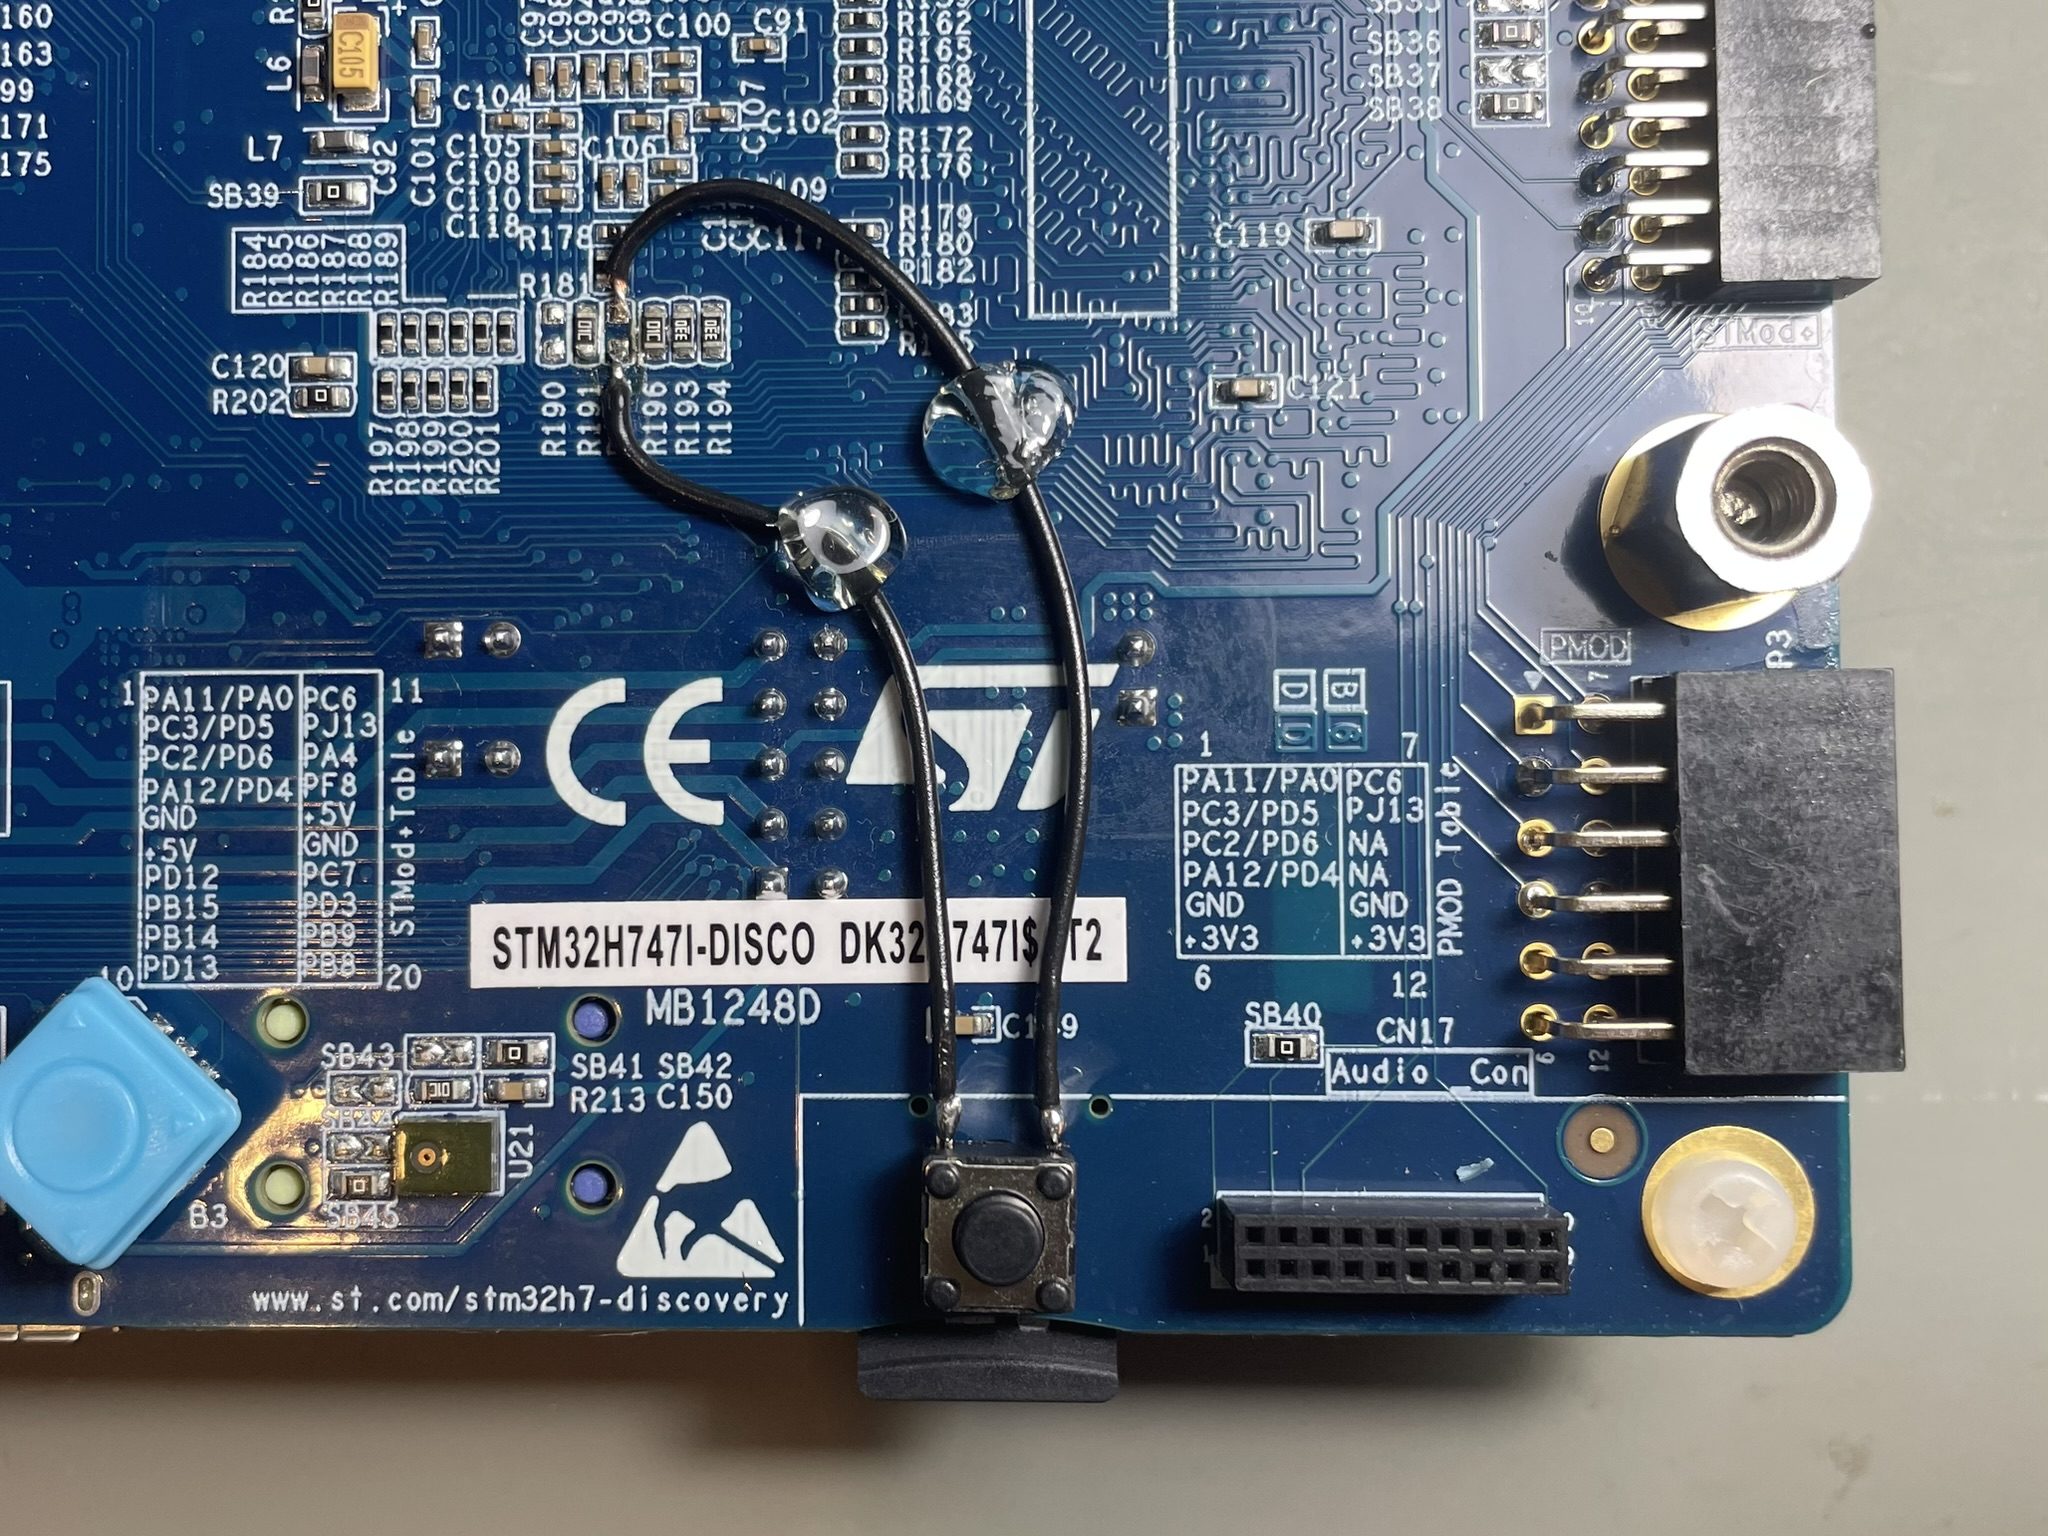
\includegraphics[width=10cm]{Resources/HW_Boot_MOD.JPEG}
	\caption{Hardware Boot Button Mod}
	\label{fig:Hardware Boot Button Mod}
\end{figure}

Later it turned out, that those problems came from a faulty RCC configuration. That's something I should investigate further. Because right now I'm only able to get up to 400MHz for the CM7. This probably has something to do with the SMPS and Voltage scaling option in the RCC tab.

\section{QSPI Flash}
To extend the internal flash of the MCU, there is 128MB of QSPI Flash on the DevBoard. In this section I'll try to implement this flash, so I'm able to store the actual firmware on this external flash. This also means, that the MCU should then boot from the external memory.

\subsection{Write Test}
In this first test I'll try to simply write some data to the Flash and therefore confirm, that the communication between the MCU and flash works as intended. For this I've again followed the instructions from Controllers Tech on YouTube. 
\cite{YT_CT_QSPI}

\begin{enumerate}
	\item Enable QSPI block in "Dual Bank with Quad Lines" mode (Because DevBoard uses two ICs, each 512Mbit) for CM7.
	\item Set up pins according to the schematics. (standard cube config is wrong.) Configure Pins to CM7 in "very high" speed mode.
	\item Enable chip select 1 for both banks.
	\item Set clock prescaler to 2. (200MHz Clock divided by 2 to the power of 2 \(\rightarrow\) 50MHz ) (Flashs max. frequency in DTR mode (dual bank) is 90MHz)
	\item Fifo threshold to 4.
	\item Sample shifting to "Sample Shifting Half Cycle"
	\item Flash size to 26. (Flash size is 2 to the power of 26 + 1 Bytes. \(\rightarrow\) 128MB )
	\item Chip select high time to "6 Cycles"
	\item For Cortex-M7 Enable: ICache and DCache.
	\item Generate code.
	\item Then add user code lines from STM GitHub. \cite{GIT_DRIVER_QSPI_FLASH} to qspi.c and qspi.h.
\end{enumerate}

Now you can download the firmware to the MCU. And verify, that no error is triggered. (Orange LED blinking) Then to verify, that the string was written to the flash: open STM32CubeProgrammer and enable the external loader for the H747-Disco DevBoard. Now at the address 0x90000000, the string "msgOut" should be shown.

\lstset{language=C,caption={QSPI Write Test CM7},label=DescriptiveLabel, style=mystyle}
\begin{codeblock}
	\lstinputlisting{../../../6_Software/qspi flash/CM7/Core/Usercode/usermain_CM7.c}
\end{codeblock}

While playing a bit with this code, I've noticed, that the flash can't manipulate single bits. It can just turn a 1 into a 0 but nor in reverse. To set a 0 to a 1 you have to erase a whole sector or the whole chip. After some research on this topic I've learned, that this behaviour is common for flash memories, as they're normally only used to store data over a long time. For example: Firmware.



\subsection{Boot from QSPI}
\label{ssec:bootfromQspi}
After trying to boot from the QSPI flash, I decided to change my plans an go on without a bootloader and external RAM. At the moment I don't know to less debug the problems I've had and therefore I decided to go on with the easier tasks of this project like the actual measurements and move the Memories implementation to another project.



\section{User Interface}
I first tried to use TouchGFX to design an embedded UI using STMs TouchGFX which is a code generator for graphical displays with STM32 microcontrollers. But it turned out, that it's a lot more complicated that I originally thought. This is due to the usage of FreeRTOS and C++, which I both didn't know by then. So also because of the limited time I decided to make a tkinter app in python to show the measured values. The app is in the software folder and has the name "CircuitVoyager UI". As a base I used the following GitHUB repo: \cite{Python_Serial_Port_Tkinter_GUI}